\cotefile{2}
\scanpage{2}
\deleted{\unsure{Formulaire} \unsure{sur|pour}\\
\unsure{variétés}\\
\unsure{Énoncé} de RR}

\fbox{\begin{minipage}{.38\textwidth}
\unsure{Classé} \unsure{parmi} les\\
\unsure{cours}.
\end{minipage}}

\margin{1}
\scanpage{3}
$X$ courbe non singulière

$\mathcal E$ anneau des classes de faisceaux cohérents mod les
$(\underline F)-(\underline F')-(\underline F'')$, \unsure{rel les|relts}
\inserted{\unsure{i.e.} suite exacte $0\to F'\to F\to F''\to0$.}
\unsure{aux} $F$ à support \uline{discret}

$\mathcal E_0$ noyau de l'augmentation (rang)

$D$ sous-anneau engendré par les faisceaux \deleted{\unsure{définis}} du type $k_x$

$D=$ groupe des diviseurs. $*$ C'est l'\uline{annulateur de $\mathcal E_0$}, donc un idéal

$N$ sous-groupe de $\mathcal E$ engendré par les
$(\underline F)-(\underline F')-(\underline F'')$

$D\cap N$ \deleted{\illegible{1}} diviseurs ``\unsure{f}-équivalents'' à $0$,
\deleted{\illegible{1}}\inserted{identiques à}

$L$ groupe des diviseurs équivalents à $0$

$\Phi$ sous-algèbre de $\mathcal E$ engendrée par les \deleted{\unsure{de}} faisceaux loc. libres

$\simeq$ algèbre des classes de fibrés vectoriels, on a

$\Phi_N$ \unsure{Quotient} de $\Phi$ par le sous-groupe ($=$ idéal) engendré par les
$c(E)-c(E')-c(E'')$
\[
*\quad \mathcal E=\Phi+D\qquad \Phi\cap D=0
\]
\[
*\quad \mathcal E/N\simeq\Phi/\Phi_N\simeq \unsure{Z|\mathbb Z}+\unsure{\mathfrak P|\mathfrak D}^{(1)}
\]
\deleted{$*\quad\unsure{D_f\subset D_0}$\quad \unsure{diviseurs} \illegible{2}\\
\unsure{défini} \illegible{2}}

\uline{Proposition} $N$ est engendré par les $c(E)-c(E')-c(E'')$, où
$0\to E'\to E\to E''\to0$ est une suite exacte de fibrés \uline{vectoriels}, et
les $c(E)-c(F)-c(\underline O_x(E)/f\underline O_x(F))$, où $E$ et $F$ sont des fibrés
\uline{linéaires} et $f:F\to E$ un \unsure{hom} non nul,
\unsure{i.e.} $f\in H^0(X,\underline O_x(F^*\otimes E))$.

Ces derniers éléments sont aussi ceux de la forme
$\lambda(D+D')-\lambda(D')-D$ \deleted{\illegible{1}}
($D$ et $D'$ diviseurs\deleted{\illegible{1}}),
$\lambda(\Delta)$ est la classe du faisceau associé au fibré vectoriel associé au diviseur $\Delta$.
On peut se borner à $D\geq0$

\margin{$(1)$ $\unsure{Z|\mathbb Z}+\unsure{\mathfrak P|\mathfrak D}\to\mathcal E/N$ fait correspondre à $(1,0)$ la classe de
$\underline O_x$, et sur $\unsure{\mathfrak P|\mathfrak D}$ se définit par passage au quotient de l'inclusion
$D\subset\mathcal E$}

\margin{\unsure{LINEN TYPEWRITER}\quad
\figure{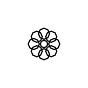
\begin{tikzpicture}[scale=.13]
\foreach \a in {0,45,...,315}{\draw (\a:1) circle (.54);}
\draw (0,0) circle (.36);
\end{tikzpicture}}\quad \unsure{ARGENTINA}}

\margin{2}
\scanpage{4}
L'assertion précédant la proposition est équivalente aux suivantes
\[
\begin{aligned}
D+N&=\mathcal E_0\\
D\cap N&=L\\[4pt]
\Phi+N&=\mathcal E\qquad\deleted{\unsure{annulation}}\\
\Phi\cap N&=\Phi_N
\end{aligned}
\]

Définition de l'application $\mathcal E\longrightarrow \unsure{Z|\mathbb Z}+\unsure{\mathfrak P|\mathfrak D}$

sur $D$ : coïncide avec l'application \uline{canonique} $D\mathrel{\text{---}}\unsure{\mathfrak P|\mathfrak D}$

sur $\Phi$ : Soit $E$ un fibré vectoriel, fibre type $K^n$ et de classe de Chern
$c^1(E)\in\unsure{\mathfrak P|\mathfrak D}$, on prend
\[
h(E)=(n,c^1(E))
\]

Soit $F$ un faisceau algébrique cohérent, $c(F)\in \unsure{Z|\mathbb Z}+\unsure{\mathfrak P|\mathfrak D}$,
\unsure{je} dis que
\[
(1)\qquad \unsure{\chi|\xi}(F)=K_1\bigl(c(F).(1-\tfrac12 K)\bigr)
\qquad (K\in\unsure{\mathfrak P|\mathfrak D})
\]
où $K$ est la classe canonique ; $K_1$ est la forme linéaire sur
$\unsure{Z|\mathbb Z}+\unsure{\mathfrak P|\mathfrak D}$ égale à $0$ sur $\unsure{Z|\mathbb Z}$, et sur
$\unsure{\mathfrak P|\mathfrak D}$ : l'application ``degré''
$\unsure{\mathfrak P|\mathfrak D}\to \unsure{Z|\mathbb Z}$.
Pour vérifier (1), il suffit de la vérifier pour $F=k_x$ et pour $F=\underline O_x$

\diagram{\begin{tikzcd}[row sep=large,column sep=large,
execute at end picture={
\draw[decorate,decoration={brace,amplitude=5pt}]
(d.east) -- (e.north west) node[midway,above right] {$\Phi$};
\draw[decorate,decoration={brace,mirror,amplitude=5pt}]
(n.south east) -- (e.south) node[midway,below right,align=center] {$\mathcal E/N$ classes de\\faisceaux};
}]
& |[alias=d]| D \arrow[dr] & & \\
L=D\cap N \arrow[ur,"\unsure{\mathfrak P|\mathfrak D}"] \arrow[dr,"?"'] & & D+N=\mathcal E_0 \arrow[r,"\mathbb Z"'] & |[alias=e]| \mathcal E\\
& |[alias=n]| N \arrow[ur] & &
\end{tikzcd}}

\margin{\unsure{LINEN TYPEWRITER}\quad
\figure{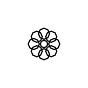
\begin{tikzpicture}[scale=.13]
\foreach \a in {0,45,...,315}{\draw (\a:1) circle (.54);}
\draw (0,0) circle (.36);
\end{tikzpicture}}\quad \unsure{ARGENTINA}}

\margin{3}
\scanpage{5}
$X$ \unsure{préschéma} [noethérien] \deleted{avec}\inserted{admettant}
Module inversible ample, $\dim X\leq1$

$K^\bullet(X)$ augmenté sur $H^0(X,Z)=Z^{\pi_0(X)}$, $E\longmapsto(\operatorname{rg}_i(E))_{i\in\pi_0(X)}$
\[
\left.\begin{gathered}
\text{L'idéal d'augmentation }\inserted{I(X)}\text{ est de carré nul}\\
\text{Si }x\in I(X),\text{ on a }\gamma^i(x)=0\text{ pour }i\geq2
\end{gathered}\right\}\quad F^i_\gamma(K^\bullet(X))=0\text{ si }i\geq2
\]
Donc
\[
K^\bullet(X)\simeq Z^{\pi_0(X)}\times K^1(X)
\]
\inserted{comme $\lambda$-anneau augmenté,}
\margin{$K^{(1)}(X)\simeq\operatorname{Pic}(X)=\prod_{i\in\pi_0(X)}\operatorname{Pic}(X_i)$
\inserted{$\simeq\deleted{\unsure{K}}\prod_{i\in\pi_0(X)}K^{(1)}(X_i)$}}

\deleted{\unsure{donc E}} $K^\bullet(X)$ entièrement déterminé (à isom près) par le système des
$\operatorname{Pic}(X_i)$, $i\in\pi_0(X)$

Si $E$ est un \deleted{fibré vectoriel}\inserted{faisceau loc libre} de rang $\unsure{n}$ sur $X$,
\unsure{on a donc|on a alors}
\[
\operatorname{cl}(E)=[\operatorname{rg}(E),c^1(E)]\qquad\text{où }c^1(E)=\det(E)
\]
\inserted{$\operatorname{rg}(E)=(\operatorname{rg}_i(E))_{i\in I}$}
\[
\left[\text{i.e.}\quad
\operatorname{cl}(E)=\sum_i\operatorname{rg}_i(E).1_i+[\operatorname{cl}(\det E)-1]
=\sum_i(\operatorname{rg}_i(E)-1)1_i+\operatorname{cl}(\det E)\right]
\]

\unsure{Car|Or}
\[
B^\bullet(X)=Z^{\pi_0(X)}\times\operatorname{Pic}(X)
\]
\diagram{\begin{tikzcd}
K^\bullet(X) \arrow[r,"c"] & B^\bullet(X)
\end{tikzcd}}
est l'identité, avec les identifications précédentes

\margin{$c$}

$K_\bullet(X)$ augmenté sur $Z^{\pi'_0(X)}$
\[
F\longmapsto(\operatorname{lg}_i(F))_{i\in\pi'_0(X)}
\]
\margin{$[\unsure{\pi^{(1)}(X)|\pi_0^{(1)}(X)}=$ ens des composantes irréductibles \uuline{de dim 1}$]$}

Le noyau est $K_0(X)$, il est isomorphe à
\[
Z^{\unsure{\pi_0^{(0)}(X)}}\times\underbrace{\operatorname{Pic}'(X)}
=Z^{\unsure{\pi_0^{(0)}(X)}}\times
\prod_{i\in\underbrace{\pi_0^{(1)}(X)}_{\substack{\text{ens des}\\\text{comp. conn.}\\\text{de }\uline{\text{dim 1}}}}}K_0(X_i)
\]

\margin{4}
\scanpage{7}
Pour écrire les opérations de $K^\bullet(X)$ sur $K_\bullet(X)$
\inserted{et l'élément \deleted{\unsure{e}} $1$ de $K_\bullet(X)$}, on
\unsure{pourra} supposer (pour simplifier l'écriture)
$X$ \uline{connexe}.

\deleted{$\unsure{K}$} $1^\circ)$ $\dim X=0$
\diagram{\begin{tikzcd}
K^\bullet(X) \arrow[r,"\operatorname{rg}","\simeq"'] & Z\\
K_\bullet(X) \arrow[r,"\operatorname{lg}"] & Z
\end{tikzcd}}
\margin{isom de $\lambda$-anneaux}

Les opérations de $K^\bullet(X)$ sur $K_\bullet(X)$ : \unsure{pas} le choix !

$1\in K_\bullet(X)$ donné par
\[
\operatorname{lg}(1)=\begin{tikzpicture}[baseline=(mu.base)]
\node[draw,ellipse,inner sep=3pt] (all) {$\phantom{\mu_i\in Z}$};
\node at (all.center) {$\phantom{\mu_i}\in Z$};
\node[draw,ellipse,inner sep=2pt] (mu) at ([xshift=-.38cm]all.center) {$\mu_i$};
\end{tikzpicture}
\]
seul invariant de la situation

ici $c^\bullet=\operatorname{ch}^\bullet=\operatorname{id}_{K^\bullet}$
\deleted{$\unsure{\mu=\operatorname{lg}}\unsure{1}$}
$c_\bullet=\operatorname{ch}_\bullet=\operatorname{id}_{K_\bullet}$

$2^\circ)$ $\dim X=1$. On a les invariants suivants

\unsure{c)} L'ens fini $\kappa=\kappa(X)$ des comp. irréd. de $X$

\unsure{e)} La famille $(\mu_i)_{i\in\kappa}$ (des $\operatorname{lg}_i(\underline O_X)$)
\inserted{$\delta\in K_0\unsure{(X)}$\qquad $(=1-\sum\mu_i1_i)$}
\margin{\unsure{un vecteur}, \unsure{dépendant du} splitting choisi
la classe résiduelle de l'élément $1$ de $K_\bullet(X)$}

$a)$ Le groupe $K^{(1)}=\operatorname{Pic}(X)$

$b)$ Le groupe $\unsure{K_{(0)}^\kappa|K_{(0)}}=K_{(0)}(X)$
\deleted{$\unsure{i\in\kappa}\ [\unsure{K_{(0)}=\prod_{i\in\kappa}K_{(0)}^i}$}

$d)$ L'\deleted{\unsure{es}}hom
\diagram{\begin{tikzcd}
u_i:K^{(1)} \arrow[r] & \unsure{K_{(0)}^\kappa|K_{(0)}}
\end{tikzcd}}
\deleted{$\unsure{i\in\kappa}$} $i\in\kappa$

(savoir \deleted{$u:K^{(1)}\longrightarrow\unsure{K_{(0)}}$}
$L\longmapsto\operatorname{cl}((\underline L-1)\underline O_{X_i})$]

Avec cela, on écrit
\diagram{\begin{tikzcd}[column sep=large]
K^\bullet(X)\simeq Z\times K^{(1)} \arrow[r,"c=\operatorname{ch}","=\operatorname{id}"'] & B^\bullet(X)\simeq Z\times K^{(1)}\\
K_\bullet(X)\simeq Z^\kappa\times K_{(0)} \arrow[r,equal,"\deleted{\unsure{\longrightarrow}}"] & B_\bullet(X)\simeq Z^\kappa\times K_{(0)}
\end{tikzcd}}
\margin{isom ``naturel'' [compatible avec changement de base]}
\margin{$K^{(1)}$ : carré nul}
\margin{isom \uline{non naturel}\\
les $\unsure{\underline O_{X_i^{\mathrm{red}}}}$ ne sont pas inv. par changement de base.}

Opérations de $K^\bullet(X)$ sur $K_\bullet(X)$ : il suffit pour
$\forall\ \xi\in K^{(1)}$ de définir dans $K_\bullet(X)$ une opération
\deleted{de carré nul, \unsure{d'élevant la} filtration \unsure{de} $1$}
de degré filtrant $\geq1$ [donc de carré nul]
i.e. un hom $Z^\kappa\longrightarrow K_{(0)}$
\deleted{$\unsure{\prod_{i\in\kappa}K_{(0)}^i}$}, on prend
\[
(l_i)_{i\in\kappa}\longmapsto(l_i u_i(\xi))_{i\in\kappa}
\]

\margin{6}
\scanpage{8}
Hom de $K^\bullet(X)$ dans $K_\bullet(X)$, défini par $1_\bullet\in K_\bullet(X)$
défini par
\[
1_\bullet=\sum\mu_i1_i+\unsure{\delta_i|\delta}
\]
Alors on aura
\[
u(\underset{\substack{\uparrow\\Z}}{n},\underset{\substack{\uparrow\\K^{(1)}}}{\xi})
=\sum n\mu_i1_i+\left(n\unsure{\delta_i|\delta}+\sum\mu_i u_i(\xi)\right)
\]
\margin{$\unsure{u}$}

\deleted{\unsure{On se définit un hom}}
\diagram{\begin{tikzcd}
\deleted{K_\bullet(X)} \arrow[r,"\deleted{c_\bullet=\operatorname{ch}_\bullet}"] & \deleted{B_\bullet(X)}
\end{tikzcd}}
\deleted{$c_\bullet(\xi_\bullet)=\deleted{\unsure{\xi}}\bigl[(\operatorname{lg}_i(\unsure{\xi_\bullet})),\xi_\bullet-\sum\operatorname{lg}_i(\unsure{\xi_\bullet})1_i-$}

\margin{7}
\scanpage{9}
Contre-exemples ---

\margin{8}
\scanpage{10}
\[
\underline K(X\times P^r)=\underline K(X)\otimes\underline K(P^r)\quad/\quad \xi=1-L^{-1}.
\]
\diagram{\begin{tikzcd}
X \arrow[r,dash,"i"] & X\times P^r
\end{tikzcd}}
\[
F\otimes L
\]
\[
i_!(x)=p^!(x)\otimes q^!(\xi^r)=x\otimes\xi^r
\]
\[
\widetilde C(i_!(x))=\widetilde C(x\otimes\xi^r)=\widetilde C(x)*\widetilde C(\xi^r)
\]
\figure{\begin{tikzpicture}[x=1cm,y=1cm]
\node[anchor=west] at (0,0) {$\displaystyle\xi^r=\sum_{i=0}^r\binom ri(-1)^iL^{-i}$};
\node at (3.2,.75) {$\deleted{\widetilde C}$};
\draw (-.2,.62) .. controls (1.4,.54) and (3.7,.93) .. (5.5,.82);
\draw (-.15,.15) -- (.38,-1.05);
\end{tikzpicture}}

\diagram{\begin{tikzcd}
\underline K(X) \arrow[r,"\text{\uuline{injectif}}"] \arrow[d,"\widetilde C_X"'] & \underline K(X\times P^r) \arrow[d,"\widetilde C_{X\times P^r}"]\\
\widetilde A(X) \arrow[r] & \widetilde A(X\times P^r)
\end{tikzcd}}
\[
p^{\deleted{\unsure{!}}}_*i_*(x)=(pi)_*x=x
\]
\figure{\begin{tikzpicture}[x=1cm,y=1cm]
\node[anchor=west] at (5.3,0) {$\displaystyle\widetilde C(\xi^r)=\prod_{i=0}^r(1-i\eta)^{(-1)^i\binom ri}$};
\node[anchor=west] at (5.0,-1.5) {$\displaystyle\widetilde C(i_!(x))=\prod_{i=0}^r[\widetilde C(x)*(1-i\eta)]^{(-1)^i\binom ri}$};
\node[anchor=west] at (6.9,-2.8) {$\deleted{=\displaystyle\prod_{i=0}^r\bigl[(1-i\unsure{\xi|\eta})^{\varepsilon(x)}\sum_{i=0}^\infty C^i(x)}$};
\draw (5.35,.65) -- (12.9,1.0);
\draw (5.15,.48) .. controls (5.1,-1.4) and (5.23,-2.9) .. (5.45,-3.55);
\draw (12.88,.64) .. controls (13.05,-.2) and (12.8,-2.2) .. (12.6,-2.9);
\draw (7.3,-3.28) .. controls (8.9,-3.25) and (11.7,-3.2) .. (13.3,-3.0)
 .. controls (13.8,-2.9) and (13.7,-3.2) .. (13.3,-3.3)
 -- (9.65,-4.0) .. controls (9.1,-4.1) and (11.2,-6.7) .. (11.55,-7.25)
 .. controls (11.75,-7.65) and (11.8,-8.1) .. (11.45,-8.2)
 -- (7.6,-8.25) .. controls (7.0,-8.2) and (7.25,-7.7) .. (7.35,-7.35);
\draw (0,-3.85) .. controls (2.8,-4.0) and (6.8,-3.45) .. (8.95,-3.55);
\node[anchor=west] at (.55,-4.25) {$\displaystyle\widetilde C(x)*(1-i\eta)=\widetilde C(x)*[1,1-i\eta]-\widetilde C(x)$};
\node[anchor=north west] at (2.7,-4.7) {$\displaystyle=\biggl[\varepsilon(x),1+\cdots+
\underbrace{\sum_{j=0}^h C^{\unsure{j}}\deleted{\unsure{\xi}}(x)(-i\eta)^{h-j}}_{
\substack{\text{\unsure{h.ième} terme }C^h\\\text{de la série}\\\widetilde C(x)*[1,1-i\eta]}}$};
\draw (.6,-4.12) -- (.6,-5.75) .. controls (2,-5.6) and (3.4,-5.55) .. (3.95,-5.9)
 .. controls (4.25,-6.1) and (3.95,-6.7) .. (4.45,-6.85)
 .. controls (5.3,-7.0) and (8.1,-7.05) .. (9.7,-7.25);
\end{tikzpicture}}

\[
\widetilde C(\xi^r)=1+(-1)^{r-1}(r-1)!\eta^r
\]
d'où
\[
\widetilde C(i_!(x))=\widetilde C(x)*(1+(-1)^{r-1}(r-1)!\eta^r)
\]
\deleted{\unsure{D'où}}
\[
=\bigl(1+(-1)^{r-1}(r-1)!\eta^r\bigr)^{\varepsilon(x)}
\underbrace{\left(C(x)*\left(1+\overbrace{(-1)^{r-1}(r-1)!\eta^r}^{\alpha^r}\right)\right)}_{
1+\sum_{i=\unsure{1}}^\infty Q_i(C^1(x),\mathrel{\text{---}}C^i(x);0\mathrel{\text{---}}0\,\underset{\substack{\text{\unsure{r.ième} argument}\\\text{après le ;}}}{\uuline{\alpha^{(r)}}},0\mathrel{\text{---}}0)}
\]
\margin{$\underline O_{\unsure{Y|y}}=1-L(-\unsure{Y|y})$\\
$1-\underline O_{\unsure{Y|y}}=L(-\unsure{Y|y})$}

Or $Q_i$ n'a pas de terme ne contenant pas un des \unsure{$c^j$}.

\margin{9}
\scanpage{11}
\margin{10}

- 12 -\hfill n° 234

6. \uline{Extensions aux puissances tensorielles et extérieures.}

Supposons $A$ \uline{commutatif}, et soit $T^p(E)$ le $A$-module puissance tensorielle $p$-ème de $E$ (chap.III,\S\S1 et 4). Pour toute application semi-linéaire $u$ (relative à $J$) de $E$ dans un $A$-module $F$, il existe une application semi-linéaire et une seule $u'$ (relative à $J$) de $T^p(E)$ dans $T^p(F)$, telle que
\[
(18)\qquad u'(x_1\otimes x_2\otimes\ldots\otimes x_p)=u(x_1)\otimes u(x_2)\otimes\ldots\otimes u(x_p)
\]
Cela se voit en tenant compte de la définition du produit tensoriel, exactement comme pour le cas où $u$ est linéaire (si $v(x_1,\ldots,x_p)$ est le second-membre de (18), $v$ se prolonge en une application semi-linéaire $\bar v$ (relative à $J$) du module $G=A^{(E^p)}$ des combinaisons linéaires formelles des éléments de l'ensemble $E^p$, et comme
\[
v(x_1,\ldots,\lambda x_i,\ldots,x_p)=\lambda^J v(x_1,\ldots,x_p)
\]
$\bar v$ s'annule pour tous les éléments de $G$ de la forme
\[
(x_1,\ldots,\lambda x_i,\ldots,x_p)-\lambda(x_1,\ldots,x_p)\ ;
\]
cf.chap.III,\S1,n°2). Appliquons ce résultat aux applications semi linéaires $f$ et $g$ de $E$ dans $\unsure{E|E^*}$, associées à une forme sesquilinéaire $\Phi$ ; on obtient deux applications semi-linéaires de $T^p(E)$ dans $T^p(E^*)$ ; désignons par $f_p,g_p$ les applications semi-linéaires obtenues en composant avec ces applications, l'application canonique de $T^p(E^*)$ dans le dual $(T^p(E))^*$ (chap.III,\S1,n°4) ; on a par définition
\[
\begin{aligned}
\langle x_1\otimes\ldots\otimes x_p,f_p(y_1\otimes\ldots\otimes y_p)\rangle
&=\langle x_1,f(y_1)\rangle\ldots\langle x_p,f(y_p)\rangle\\
&=\Phi(x_1,y_1)\ldots\Phi(x_p,y_p)
\end{aligned}
\]
et de même
\[
\langle y_1\otimes\ldots\otimes y_p,g_p(x_1\otimes\ldots\otimes x_p)\rangle^J
=\langle y_1,g(x_1)\rangle^J\ldots\langle y_p,g(x_p)\rangle^J=
\]
\scanpage{12}
Or $Q_i$ n'a \deleted{\unsure{aucun}}\inserted{pas de} terme ne contenant aucun des arguments après la virgule;
en plus, notons que $(\eta^r)^n=0$ si $n>1$. Donc on trouve
\[
Q_i(\text{---})=\begin{cases}
0&\text{si }i<r\\
(-1)^{r-1}(r-1)!\,Q_{i-r}^{(r)}(c^1(x),\text{---}\,c^i(x))
\end{cases}
\]
où $Q_{i-r}^{(r)}(c^1\deleted{\unsure{(x)}},\text{---},c^i\deleted{\unsure{(x)}})$
est le coefficient de $d^r$ dans $Q_i(c^1,\text{---}\,c^i;d^1,\text{---}\,d^i)$.
$(r\leq i)$.
\inserted{(est un \unsure{pol. isob.} de poids $i-r$)}
Ainsi on trouve, tenant compte que $(\eta^r)^n=0$ pour $n>1$
\[
\widetilde C(i_!(x))=1+(-1)^{r-1}(r-1)!\eta^r
\left[\varepsilon(x)+\sum_{i=0}^\infty Q_i^{(r)}(c^1(x),\text{---}\,c^i(x))\right]
\]
\unsure{Comparons|Convenons} \unsure{avec|pour} R.R.
\[
\widetilde C(i_!(x))=\deleted{\unsure{\widetilde C}}(i_*)_r(\widetilde C(x))
\]
\unsure{on écrit} \unsure{que}
\[
(i_*)_r\left[n,\sum_0^\infty x^i\right]
=1+(-1)^{r-1}(r-1)!\eta^r\biggl[n+\sum_{i=0}^\infty Q_i^{(r)}(x^1\text{---}x^i)
\]

N.B. $Q_0^{(r)}(c^1,\text{---}\,c^r)=0$, i.e.
$Q_r^{\unsure{*}}(c^1\text{---}c^r;0,\text{---}\,0,d^r)=0$

i.e. $(1+c^1+\text{---}+c^r)*(1+d^r)$ est de filtration $\geq r+1$

\unsure{De m.}, on voit
\[
\uuline{Q_1^{(r)}(c^1)}\deleted{\unsure{c^2}}
=-\frac{(r+1-1)!}{(r-1)!(1-1)!}\,c^1=\uuline{-rc^1}
\]

On fera attention que, par suite, s'il y a de la torsion dans $A(X)$,
l'hom $(i_*)_r$ est non injectif, à cause de \unsure{ses|les} coefficients numériques
(\unsure{dus tant} à $(r-1)!$ \unsure{qu'à ceux} provenant des $Q_i^{(r)}$

\margin{11}
\scanpage{13}
\margin{12}

- 10 -\hfill n° 234

5. \uline{Matrice d'une forme sesquilinéaire.}

Supposons que $E$ admette une base finie $(e_i)_{1\leq i\leq n}$, et posons
$\rho_{ij}=\Phi(e_i,e_j)$. On a
\[
(15)\qquad
\Phi\left(\sum_{i=1}^n\xi_i e_i,\sum_{i=1}^n\eta_i e_i\right)
=\sum_{i,j}\xi_i\rho_{ij}\eta_j^J.
\]
Inversement, soit $(\rho_{ij})_{1\leq i\leq n,\ 1\leq j\leq n}$ une
\deleted{famille d'}\inserted{matrice à} éléments \deleted{de}\inserted{dans} $A$
et définissons $\Phi$ par la formule (15). Il est immédiat que $\Phi$ est une forme sesquilinéaire sur $E$.
La matrice carrée $\mathcal R=(\rho_{ij})$ à éléments dans $A$, est appelée
\uline{la matrice de $\Phi$ par rapport à la base} $(e_i)$.

Dans tout ce qui suit, pour toute matrice (rectangulaire) $\mathcal U=(\lambda_{ij})$ à éléments dans $A$, nous poserons $\mathcal U^J=(\lambda_{ij}^J)$.
Si on désigne par $x$ et $y$ les matrices à une colonne ayant comme éléments respectifs les $\xi_i$ et les $\eta_i$ $(1\leq i\leq n)$, la formule (15) peut encore s'écrire
\[
(16)\qquad \Phi(x,y)={}^t x.\mathcal R.y^J.
\]

Soient $F$ un second $A$-module à gauche admettant une base finie $(f_j)_{1\leq j\leq m}$,
$u$ une application linéaire de $F$ dans $E$, et posons
$u(f_j)=\sum_{i=1}^n\lambda_{ij}e_i$. Soit $\Phi'$ la transformée de $\Phi$ par $u$, et posons
$\rho'_{ij}=\Phi'(f_i,f_j)$ $(1\leq i\leq m,1\leq j\leq m)$. On a
\[
\rho'_{ij}=\Phi\left(\sum_{k=1}^n\lambda_{ki}e_k,\sum_{k=1}^n\lambda_{kj}e_k\right)
=\sum_{h,k}\lambda_{hi}\rho_{hk}\lambda_{kj}^J
\]
de sorte que, si $\mathcal U$ est la matrice $(\lambda_{ij})$ à $\unsure{m|n}$ lignes et $\unsure{n|m}$ colonnes,
la matrice $\mathcal R'=(\rho'_{ij})$ de $\Phi'$ par rapport à $(f_j)$ est donnée par
\[
(17)\qquad \mathcal R'={}^t\mathcal U.\mathcal R.\mathcal U^J.
\]

Dans cette formule, les matrices ${}^t\mathcal U$ et $\mathcal U^J$ doivent être considérées comme ayant leurs éléments dans $A$ (chap.II,\S6,n°6) ; il en est de même les matrices ${}^t x$ et $y^J$ dans (16).
\scanpage{14}
\deleted{\unsure{Comme}}
\deleted{Soit donc $Y$ une hypersurface \deleted{\unsure{non irréductible}}\inserted{à composantes disjointes} dans $X$.
\inserted{$x^1\in A^1(X)$ sa classe}
On a
\[
\widetilde C_X(Y)=(1-\deleted{\unsure{d(Y)}}x^1)^{-1}=\sum x^{1n}
\]
\[
\begin{aligned}
\widetilde C_{X\times P^r}(i_!(\underline O_Y))
&=\widetilde C_{X\times P^r}(Y\times P^r)\\
&=\deleted{1+(-1)^{r-1}(r-1)!\sum_{i=1}^\infty Q_i^{(r)}(x^1,(x^1)^2\text{---}\unsure{x^i})}\\
&\quad1+(-1)^{r-1}(r-1)!\eta^r\sum_{i=1}^\infty
\underbrace{Q_i^{(r)}(x^1,(x^1)^2,\text{---}\,(x^1)^{\unsure{r|i}})}_{C_{i,r}(x^1)^{\unsure{r|i}}}
\end{aligned}
\]
\deleted{$1+\sum$}
Si donc $(r-1)!X^1=0$, on a $\widetilde C_{X\times P^r}(Y\times P^r)=0$,
sans que pourtant l'on ait nécessairement $X^1=0$.
Cas le plus simple : $r=3$, $X$ une courbe elliptique.}

\uline{N.B.} Il se peut qu'on ait un élément $x$ de $\underline K(X)$ tel que les
$\unsure{C^i|c^i}(x)$ sont tous annulés par $(r-1)!$, sans que $x$ soit nul.
Alors $y=i_!(x)$ a la propriété que $\widetilde C(\deleted{\unsure{x}}\inserted{y})=0$,
mais $y\ne0$. Exemple le plus simple :

$X=$ courbe elliptique, $\inserted{x\in\underline K(X)}$ \unsure{classe} de diviseur \unsure{non}
nul d'ordre $2$, [p.ex. $x=(a)-(0)$, où $a\in X$ est tel que $a+a=0$, $a\ne0$], et $r=3$.
\uline{On a donc dans $P^3\times X$ la différence de deux $\unsure{V^0|V^s}$
\deleted{\unsure{points}} dont la classe de Chern est nulle ; sans qu'elle soit nulle.}

\margin{13}
\scanpage{15}
\margin{$-9-$\qquad N$^\circ$ 234}
considéré comme espace vectoriel à droite sur $\varphi(A)$), et les $x_i\ne0$ appartiennent à $E$. Pour tout $y\in E$, on a alors la relation $\unsure{\Phi'|\Phi^\circ}(x',1\otimes y)=0$ qui s'écrit $\sum_{i=1}^n\alpha_i\varphi(\Phi(x_i,y))=0$, et entraîne donc $\Phi(x_i,y)=0$ pour $1\le i\le n$, d'où le corollaire.

4. \uline{Quelques identités}.

Soit $\Phi$ une forme sesquilinéaire sur $E$. Posons $\unsure{\Phi|\varphi}(x,x)=Q(x)$. On a
\[
\begin{aligned}
(9)\qquad Q(x+y)&=Q(x)+\Phi(x,y)+\Phi(y,x)+Q(y)\\
(10)\qquad Q(x-y)&=Q(x)-\Phi(x,y)-\Phi(y,x)+Q(y)
\end{aligned}
\]
d'où
\[
(11)\qquad 2(\Phi(x,y)+\Phi(y,x))=Q(x+y)-Q(x-y).
\]
Soit $\lambda\in A$ ; en remplaçant $y$ par $\lambda y$ dans (11), il vient
\[
(12)\qquad 2(\Phi(x,y)\lambda^J+\lambda\Phi(y,x))=Q(x+\lambda y)-Q(x-\lambda y)
\]
et on tire de (11) et (12)
\[
\begin{aligned}
(13)\qquad 2(\lambda\Phi(x,y)-\Phi(x,y)\lambda^J)
&=\lambda Q(x+y)-\lambda Q(x-y)-Q(x+\lambda y)+{}\\
&\qquad{}+Q(x-\lambda y).
\end{aligned}
\]
Supposons en particulier que $A$ soit une extension quadratique $K(i)$ d'un anneau commutatif $K$, avec $i^2=-1$ (chap. II, \S 7, n$^\circ$7), et que $J$ soit l'automorphisme $\alpha+\beta i\longrightarrow\alpha-\beta i$ de $A$ ; en faisant $\lambda=i$ dans (13), on obtient
\[
(14)\qquad 4\Phi(x,y)=Q(x+y)-Q(x-y)+iQ(x+iy)-iQ(x-iy).
\]
\margin{\uline{Remarque}}
On notera que les formules précédentes sont encore \deleted{applicables}\inserted{valables} si $\Phi$ est une application de $E\times E$ dans un $A$-bimodule $F$ (\uline{à gauche et à droite}), vérifiant les relations (1), (2), (3), (4).
\margin{?}
\margin{14}
\scanpage{16}
\deleted{$\unsure{\mathfrak X}$} $\mathfrak X$ Topos annelé, $O_{\mathfrak X}=O$ son anneau. (\unsure{Supposé} \unsure{comm.})

Pour tout groupe $G$, on considère la catégorie
\[
\mathcal A(\mathfrak X,G)
\]
des Modules sur $\mathfrak X$ où $G$ opère. \unsure{On a} pour un hom $u:G\mathrel{\text{---}}G'$ un hom restriction
\[
u^*:\mathcal A(\mathfrak X,G')\mathrel{\text{---}}\mathcal A(X,G)
\]
et un homomorphisme extension
\[
u_*:\mathcal A(X,G)\mathrel{\text{---}}\mathcal A(X,G').
\]
Lorsque $u$ est injectif, alors on a \deleted{\unsure{donc}} un isom \inserted{fonctoriel} \unsure{non} canonique
\[
u^*u_*(F)\simeq F^{(G'/G)}
\]
Si on se borne aux sous-catégories qui sont \unsure{formées} des Modules libres (resp. loc. libres, resp. libres de type fini, resp. loc. libres de type fini) sur $O[G]$, elles sont stables pour les foncteurs précédents. Elles le sont également pour les foncteurs qu'on va définir maintenant.

Dans $\mathcal A(\mathfrak X,G)$ \unsure{on a} l'opération $\otimes$ (comm. et associative), pour un hom $u:G\mathrel{\text{---}}G'$
\margin{15}
\scanpage{17}
on a les isom fonctoriels
\[
u^*(F'\otimes G')\simeq u^*(F')\otimes u^*(G')
\]
et pour $u_*$ on a la ``formule de projection''
\[
u_*(F\otimes u^*(G'))\simeq u_*(F)\otimes G'
\]
[On a aussi des opérations $\Lambda^i$ (et autres opérations tensorielles) \unsure{que nous allons déduire} plus bas des opérations $\otimes$]

``Produit tensoriel externe''
\[
F\boxtimes G
\]
\margin{$F\in\operatorname{Ob}\mathcal A(\mathfrak X,G),\ G\in\operatorname{Ob}\mathcal A(\mathfrak X,H)$
\[
F\boxtimes G=\operatorname{pr}_1^*(F)\otimes\operatorname{pr}_2^*(G)\in\operatorname{Ob}\mathcal A(\mathfrak X,H\times G)
\]}
Est compatible avec les images inverses
\[
(u\times v)^*(F\boxtimes G)\simeq u^*(F)\boxtimes v^*(G)
\]
et redonne $F\otimes G$ par
\[
F\otimes G=(\operatorname{diag}_G)^*(F\boxtimes G)
\]
On pose
\[
\mathcal A(\mathfrak X,p)=\mathcal A(X,\unsure{\mathfrak S}_p)\qquad p\in\mathbb N
\]
\margin{\unsure{Éventuellement} introduire aussi $\mathcal A(\mathfrak X,p_1,\ldots,p_r)=\mathcal A(\mathfrak X,\mathfrak S_{p_1}\times\cdots\times\mathfrak S_{p_r})$}
Alors tout hom $u\deleted{\unsure{f_i}}:\mathfrak S_p\longrightarrow\mathfrak S_q$ donne des foncteurs
\diagram{\begin{tikzcd}
\mathcal A(\mathfrak X,p)&\mathcal A(\mathfrak X,q)\arrow[l,"u^*"']\\
\mathcal A(\mathfrak X,p)\arrow[r,"u_*"]&\deleted{\unsure{\mathcal E}}\mathcal A(\mathfrak X,q)
\end{tikzcd}}
\inserted{avec} \uline{transitivité} pour $u$
\margin{16}
\scanpage{18}
On désigne par
\[
u_{pq}:\mathfrak S_p\times\mathfrak S_q\longrightarrow\mathfrak S_{p+q}
\]
l'injection canonique, et on pose, pour
\[
F\in\operatorname{Ob}\mathcal A(\mathfrak X,p),\quad G\in\operatorname{Ob}\mathcal A(\mathfrak X,q)
\]
\[
F*G=u_{pq*}F\boxtimes G\qquad\in\operatorname{Ob}\mathcal A(\mathfrak X,p+q)
\]
L'opération $F*G$ est ``comm'' et ``ass.'' dans un sens évident. \deleted{\unsure{On peut donc}}\inserted{\unsure{Ainsi la}} \deleted{définir} ``catégorie graduée'' $(\mathcal A(\mathfrak X,p))_{p\in\mathbb N}$ devient un ``Anneau gradué'' ; en plus les ``Structures d'anneaux'' sur les morceaux homogènes $\mathcal A(\mathfrak X,p)$ séparément.

\deleted{\unsure{Fonctorialité|Foncteurs}}
On définit d'autre part les
\[
T^n(F)=F^{\otimes n}\quad\inserted{(F\in\operatorname{Ob}\mathcal A\mathfrak X)}
\]
comme objets de $\mathcal A(\mathfrak X,n)$ ;
\deleted{plus généralement $F\in\operatorname{Ob}\mathcal A(\mathfrak X,m)$, alors $T^n(F)=F^{\otimes n}$ est un $\unsure{O}_{\mathfrak X}$-Module à groupe d'opérateurs $\mathfrak S_m\times\mathfrak S_n$, \inserted{\unsure{opère diagonalement}} et utilisant $\unsure{u_{m,n}}$ on obtient}
\margin{17}
\scanpage{19}
Formules\qquad $[F,G\in\operatorname{Ob}\mathcal A(\mathfrak X)]$
\[
T^{\unsure{n|m}}(F+G)\simeq\coprod_{p+q=n}T^p(F)*T^q(G)
\]
\[
T^m(T^n(F))\simeq w_{m,n}^*(T^{mn}(F))
\]
\[
T^{\unsure{n|m}}(F\otimes G)\simeq T^{\unsure{n|m}}(F)\otimes T^{\unsure{n|m}}(G)
\]
$[w_{m,n}:\mathfrak S_m\mathrel{\text{---}}\mathfrak S_{mn}\ \unsure{convenable}]$

Nous nous intéresserons aux $O_{\mathfrak X}(\mathfrak S_n)$-Modules $F$ ayant la propriété suivante :

$(*)$ $F$ est la somme de faisceaux
\deleted{de la forme $u_{pq*}(F_{p_1p_2\text{---}p_r})$ $(\deleted{p+q}\inserted{\sum^r p_i}=n,\ \deleted{p_i\ge0}\inserted{p_i\in\mathbb N})$, les $F_{p_1p_2\text{---}p_r}$ sont des \uline{faisceaux} \deleted{loc.} \uline{libres} sur $O_{\mathfrak X}(\mathfrak S_{p_1}\times\mathfrak S_{p_2}\times\text{---}\times\mathfrak S_{p_r})$.

On dit que $F$ est admissible s'il satisfait \uuline{loc.} la condition précédente.

(N.B. Si $F$ satisfait $(*)$, et est de type fini, il en est de $=$ des $F_{p_1\text{---}p_r}$ qui interviennent \unsure{dans} $(*)$)}
\inserted{induits par les $u_{p_1\text{---}p_r}$ et des faisceaux \inserted{\unsure{loc. libres comme|localement libres comme} $O_{\mathfrak X}$-\unsure{libres}} \uline{triviaux} sur les $\mathfrak S_{p_1}\times\text{---}\times\mathfrak S_{p_r}$}
\margin{18}
\scanpage{20}
\uline{Cas des \unsure{schémas}}

\uline{Filtration des $\lambda$-anneaux},

classes de Chern universelles

$\lambda$-anneaux ``spéciaux'' i.e. avec éléments ``géométriques''

\unsure{Applications}\quad $\unsure{\checkmark|\vee}$
\margin{19}
\scanpage{21}
$K$ $\lambda$-anneau \deleted{de \unsure{Chern} [\unsure{augmenté}]} \uline{spécial}.

$(x_s)_{s\in S}$ \deleted{\unsure{E}} \deleted{base}\inserted{famille} de générateurs (pour la structure anneau) géométriques, pour $s\in S$ soit $\varepsilon(s)=\operatorname{rg}x_s$.

On \unsure{s'intéresse} aux $\lambda$-hom $K\xrightarrow{\rho}\widetilde A$ ($A$ anneau comm. gradué) tels que $\rho^i(x_s)\unsure{=|\ne}0$ pour $i>\varepsilon(s)$.
\deleted{\unsure{Il}} il y a un pb d'applications universelles et une solution \deleted{$\unsure{\widetilde{CK}}$} $CK$, $\unsure{\widetilde c|\widetilde C}:K\longrightarrow\widetilde{CK}$.

[Ne change pas si \inserted{remplace $S$ par l'\uline{ens.} des $x_s$, ou sa \unsure{clôture}} on \unsure{clôture} $S$ par $+,\times$ et $\lambda^i$; et y ajoute $1$ \deleted{$\unsure{1}$}; --- \unsure{bien entendu} $\unsure{\mathbf1\in K|\mathbb Z\subset K}$]

\uline{Exemple} Considérons \deleted{$\mathbb Z[(X_s)_{s\in S}]=B$} le $\lambda$-anneau \inserted{spécial} $B$ engendré par des générateurs $X_s$ ($s\in S$) soumis à: \deleted{$\unsure{\lambda^i}$} ($X_s$ géométrique de rg $\varepsilon(s)$), i.e.
\[
\lambda^i(X_s)=0\quad\text{si }i>\varepsilon(s),\qquad
\lambda^{\varepsilon(s)}(X_s)\text{ est inversible}.
\]
Donc
\[
B=\mathbb Z[(\lambda^i(X_s))_{s\in S,\,1\leq i\leq\varepsilon(s)}]
[(\lambda^{\varepsilon(s)}(X_s)^{-1})].
\]
Prenons pour la famille $(X_s)_{s\in S}$. Alors on a
\[
CB=\mathbb Z[(c_s^i\deleted{(X_s)})_{s\in S,\,1\leq i\leq\varepsilon(s)}],\qquad
\widetilde{\unsure{c|C}}_B:B\mathbin{\text{---}}\widetilde{CB}\quad\text{évident}.
\]
\margin{\deleted{$B$}}
\[
\widetilde c(X_s)=[\varepsilon(s),1+c_s^1\deleted{(X_s)}\mathbin{\text{---}}\mathbin{\text{---}}c_s^{\varepsilon(s)}\deleted{(X_s)}].
\]

Il y a sur $\widetilde{CB}$ une filtration, d'où par image réciproque par $\widetilde{\unsure{c|C}}_B$ une filtration \unsure{de $\lambda$-anneau} sur $B$: compatible avec la structure d'anneau, stable pour les $\lambda^i$.
Le $\lambda$-anneau $B$ \deleted{satisfait} solution d'un pb universel, ce qui permet de définir un hom \inserted{$u$} de $\lambda$-anneaux $u$
\[
(*)\qquad
\diagram{\begin{tikzcd}
B \arrow[r,"u"] \arrow[d,"\widetilde{\unsure{c|C}}_B"'] & K \arrow[d,"\widetilde{\unsure{c|C}}_K"] \\
\widetilde{CB} \arrow[r,leftrightarrow,"\unsure{\widetilde u'|\widetilde u^!}"'] & \widetilde{CK}
\end{tikzcd}}
\]
qui par hypothèse est surjectif. L'image par $u$ de la filtration mise sur $B$ est une filtration, compatible avec la structure d'anneau, stable pour $\lambda$. On voit donc de suite que \uline{$\widetilde{\unsure{c|C}}_K$ est compatible avec les filtrations}, d'où un hom canonique
\[
\psi_K:GK\longrightarrow G\widetilde{CK}\simeq CK.
\]

\uline{Remarque} Il est facile de voir que la filtration mise sur $K$ ne dépend que de la partie $T$ de $K$ engendrée par les $x_s$ comme il a été dit. Elle a une propriété fonctorielle évidente ---

Remarquons que $K$ est augmenté (\unsure{comme pour} $B$; \unsure{cela par} $\varepsilon(X_s)=\varepsilon(s)$), $u$ compatible avec les augmentations.
\deleted{Définissons, pour $x\in K$, \unsure{$\gamma$}.}

\uline{Proposition 1} Pour $x\in K$, on a $\gamma^i(x-\varepsilon(x))\in K^{(i)}$ ($i$ quelconque $\geq0$). Posons
\[
c_K^i(x)=\deleted{\unsure{\lambda^i}}\inserted{\gamma^i}(x-\varepsilon(x))\bmod \unsure{K^{(i+1)}}\in G^i(K),\qquad
\text{donc}\quad
\widetilde{\unsure{c|C}}_K(x)=[\varepsilon(x),\unsure{\sum}_{0}^{\infty}c^i(x)].
\]
Alors $\widetilde{\unsure{c|C}}_K$ est un $\lambda$-hom. de $K$ en $\widetilde{GK}$.
Vérification immédiate! Donc $\widetilde c$ définit un hom d'anneaux gradués,
\[
\varphi_K:GK\longleftarrow CK
\]
rendant commutatif]
\[
\diagram{\begin{tikzcd}
K \arrow[r,"\widetilde{\unsure{c|C}}_K"] \arrow[dr,"c_K"'] & \widetilde{CK} \arrow[d,"\widetilde\varphi_K"] \\
& \widetilde{GK}
\end{tikzcd}}
\]
les hom. \deleted{\unsure{et les applications}} fonctoriels dans un sens évident

\uline{Proposition 2} \unsure{On} a en degré $i$:
\[
\psi_K\varphi_K=(-1)^i(i-1)!\operatorname{id};\qquad
\varphi_K\psi_K=(-1)^i(i-1)!\operatorname{id}.
\]
\margin{20}
\scanpage{22}
\uline{Démonstration} Comme $C\deleted{\unsure{B}}B\mathbin{\text{---}}CK$ et $GB\mathbin{\text{---}}GK$ sont surjectifs, on est ramené au cas de $B$.
Soit $\unsure{\xi^i|\xi}\in G^i(B)$ provenant de $P\in B^{(i)}$, on a
\[
\psi_B(\xi^i)=C_B^i(P\deleted{\unsure{(\{\lambda^i(X_s)\})}})
\]
d'où
\[
\varphi_B\psi_B(\xi^i)=\varphi_B(C_B^i(P))=c_B^i(P)
\equiv\deleted{\unsure{c_B^i}\ \text{\unsure{classe de}}}\gamma^i(P-\varepsilon(P))\bmod B^{(i+1)}.
\]
Or \unsure{on veut prouver}
\[
\gamma^i(P-\varepsilon(P))-(-1)^{i-1}(i-1)!P\in B^{(i+1)}
\]
\unsure{revient encore}, \uline{par} \uline{définition} de la filtration $B^{\deleted{\unsure{(i+1)}}}$, que l'image par $\widetilde C_B$ du premier mbr est dans $\widetilde{CB}^{(i+1)}$. Or cette image est
\[
\gamma^i(\overline P-\varepsilon(\overline P))-(-1)^{i-1}(i-1)!\overline P
\]
où $\overline P=\widetilde C_B(P)\in\deleted{\unsure{B^{(i)}}}\widetilde{CB}^{(i)}$.
Il est bien connu que \unsure{pour un tel $\overline P$}, l'expression précédente est dans $\widetilde{CB}^{(i+1)}$. On a bien prouvé
\[
\varphi_B\psi_B=(-1)^{i-1}(i-1)!\quad\text{en degré }i.
\]
On en conclut que
\[
(\psi_B\varphi_B)\psi_B=(-1)^{i-1}(i-1)!\psi_B\quad\text{en degré }i.
\]
Or l'\deleted{\unsure{espace}}\inserted{groupe-}but $CB$ de $\psi_B\varphi_B$ est sans \uline{torsion}, et le groupe image \deleted{de} $\psi_B$ dans $CB$ est $CB$ mod torsion, comme on vérifie \deleted{\unsure{très}} facilement.
\inserted{[en se ramenant au cas où $S$ est réduit à un élément ---]}
Il en résulte bien que $\psi_B\varphi_B=(-1)^{i-1}(i-1)!$, cqfd.

On voit que $\varphi_B:CB\longrightarrow GB$ est surjectif (\unsure{le cas se ramène au cas} où $S$ est réduit à un élément) donc \deleted{bijectif puisque} \inserted{$\varphi_B\psi_B=(-1)^{i-1}(i-1)!$}, et que $CB$ est sans torsion. Donc

\uline{Prop. 3} $\varphi_B$ est bijectif.

\uline{Corollaire} $\varphi_K$ est tjrs surjectif. Son noyau est un groupe de Torsion.

La première assertion résulte de ce que $GB\mathbin{\text{---}}GK$ est surjectif. La deuxième assertion résulte de $\psi_K\varphi_K=(-1)^{i-1}(i-1)!$.

\uline{Question} Est-ce que $\varphi_K$ est tjrs \uline{bijectif} ??? \uuline{Non}

\uline{Exemple} Soit \deleted{\unsure{par exemple}} $K=\mathbb Z[L]/(L-1)^n\deleted{\unsure{K}}$ ($\lambda_t L=1+Lt$), \inserted{(i.e. $K=K(P^{n-1})$)}, donc
\margin{\inserted{\uuline{un seul} générateur $X_s=L$}}
\margin{si $n-1>1$ i.e. $n\geq3$,}
\[
CK=\mathbb Z[\xi]/\text{\unsure{idéal homogène engendré par}}
\]
\[
(1+\xi)^{*n}=1+(-1)^{\unsure{n-1}}(n-1)!\xi^n+\text{---}
\]
et $CK$ a de la torsion. Cependant, \deleted{\unsure{on vérifie}} la filtration de $K$ est définie par les monômes isobares en
\[
\gamma^i(L-\varepsilon(L))=\gamma^i(L-1)
\]
qui sont \deleted{\unsure{tous}} égaux à: $L-1$ si $i=1$; à $0$ si $i>1$. Donc la filtration de $K$ est celle par les puissances de l'idéal \inserted{\uline{d'augmentation}} $(L-1)$, donc le gradué associé est sans torsion.

\margin{Mais si on adjoint à la liste géométrique $nL-1$ (qui correspond au fibré tangent à $\unsure{P(n-1)|P^{n-1}}$) on trouve $CK=\mathbb Z[\xi]/\xi^n$!}

\deleted{\uline{Proposition} (à prouver directement): Soit $K$ un $\lambda$-anneau, $(X_s)_{s\in S}$ une famille d'éléments géométriques de $K$, $K'$ le sous-$\lambda$-anneau engendré par les $X_s$, $C$ un \unsure{$\lambda$-homomorphisme} $K\longrightarrow\widetilde A$. Conditions équivalentes (i) $C^i(X_s)=0$ si $i>\varepsilon(X_s)$ (ii)}
\margin{21}
\scanpage{23}
\margin{$\unsure{=1)}$}
\[
B=\mathbb Z[(\lambda^i(X_s))_{\substack{s\in S\\1\leq i\leq\varepsilon(s)}},
(\lambda^d(Y_t))_{\substack{t\in T\\d\geq1}}]
\]
\margin{augmentation définie par les $\varepsilon(s),\varepsilon(t)$}
\[
CB=\mathbb Z[(\xi_s^i)_{\substack{s\in S\\1\leq i\leq\varepsilon(s)}},
(\unsure{\eta_t^d|\Pi_t^d})_{\substack{t\in T\\d\geq1}}]
\]
Filtration sur $B$: \deleted{\unsure{par}} $B^{(k)}=$ ss-\deleted{anneau engendré}\inserted{groupe engendré} par les
\[
P((\gamma^i(X_s-\varepsilon(X_s))),(\gamma^j(Y_t-\unsure{\varepsilon(t)|\varepsilon(Y_t)})))
\]
avec $P$ \deleted{homogène} isobare de poids $\geq k$.

\deleted{\unsure{Prop.}} \uline{Lemme} Posons $c^i(x)=\gamma^i(x-\varepsilon(x))\bmod B^{(i+1)}$. Alors
\[
x\longrightarrow\widetilde c(x)=[\varepsilon(x),1+c^1(x)\mathbin{\text{---}}]
\]
est un $\lambda$-hom de $B$ dans $\widetilde{GB}$.

En effet, $\widetilde c(x+y)=\bar c(x)\bar c(y)$ en vertu de $\gamma_t(x'+y')=\gamma_t(x')\gamma_t(y')$.
(où $x'=x-\varepsilon(x)$, $y'=y-\varepsilon(y)$). Prouvons
\[
\unsure{\widetilde c|\widetilde C}(xy)=\widetilde c(x)*\widetilde c(y)
\qquad
\left\{\begin{array}{ll}
\unsure{a)|1^\circ)} & x=1\text{ ou }y=1\quad\text{trivial}\\
\unsure{b)|2^\circ)} & x\text{ et }y\text{ d'augmentation }0.\quad\text{Alors}
\end{array}\right.
\]
\deleted{i.e. $c^i(xy)=Q_i$}
\[
\unsure{\widetilde c(xy)|c^i(xy)}=Q_i(c^1(x),\mathbin{\text{---}}c^i(x);c^1(y),\mathbin{\text{---}}c^i(y))
\]
soit encore \unsure{aut. dit}
\[
\gamma^i(xy)\equiv\uuline{Q_i}(\gamma^1(x),\mathbin{\text{---}}\gamma^i(x);\gamma^1(y),\mathbin{\text{---}}\gamma^i(y)).
\]
Or on a en effet $\gamma^i(xy)=$ polynôme à \unsure{coeff. entiers} en les $\gamma^j(x),\gamma^h(y)$, et on voit \unsure{facile} que ce polynôme est d'\uline{ordre} $\geq i$ et \deleted{\unsure{commence par} $\widetilde Q_i$}\inserted{\unsure{la comp.} de poids le plus bas est $Q_i$}
\margin{22}
\scanpage{24}
\begin{center}- 80 -\end{center}

\uline{Définition 6.} \uline{Soient} $A$ \uline{un anneau d'intégrité}, $K$ \uline{son corps des fractions}
$P^*$ \uline{le groupe ordonné des idéaux principaux fractionnaires de $K$ relativement à} $A$; \uline{on dira que} $A$ \uline{est factoriel si} $P^*$ \uline{est isomorphe à un groupe} $\unsure{\mathbf Z|\mathbb Z}^{(I)}$.

En d'autres termes, $A$ est factoriel s'il existe une famille $(p_\iota)$ d'éléments de $A$ ayant la propriété suivante: tout $x\in K^*$ peut s'écrire d'une manière et d'une seule sous la forme
\[
x=u\prod_\iota p_\iota^{n_\iota}\qquad(1)
\]
où $u$ est un élément inversible de $A$, et où les $n_\iota$ sont des entiers, tous nuls sauf un nombre fini d'entre eux, et tous $\geq0$ chaque fois que $x\in A^*$. Le groupe $P^*$ étant alors réticulé, toutes les propriétés de divisibilité démontrées en algèbre (Alg.,Chap...) concernant le pgcd, le ppcm, les éléments étrangers, etc., s'appliquent aux anneaux factoriels; la famille $(p_\iota)$ étant comme ci-dessus, il est clair que tout $p_\iota$ est un ``élément extrémal'' de $A$ (Alg.,...), et que réciproquement tout élément extrémal est de la forme $up_\iota$, où $u$ est inversible dans $A$, c'est-à-dire est associé à un $p_\iota$ et à un seul.

Dans ces conditions, $A$ est normal. En effet, pour tout $x\in K^*$, soit $v_\iota(x)=n_\iota$ l'exposant de $p_\iota$ dans l'expression (1) de $x$; et soit $v_\iota(0)=+\infty$. D'après l'unicité de (1), on a $v_\iota(xy)=v_\iota(x)+v_\iota(y)$ quels que soient $x,y$. Par hypothèse, $x\in A$ entraîne $v_\iota(x)\geq0$ quel que soit $\iota$; la réciproque est évidente. Il s'ensuit que, pour $x\in A$, $x\in\unsure{p_\iota^{n_A}|p_\iota^n A}$ est équivalent à $v_\iota(x)\geq n$; on en conclut aussitôt que, pour $x\in A$, $v_\iota(x+y)\geq\min[v_\iota(x),v_\iota(y)]$; d'après la prop.2 du § 3, n°\unsure{2}, la même propriété reste valable alors quels que soient $x,y$ dans $K$; donc les $v_\iota$ sont des valuations discrètes de $A$ et forment un ensemble de définition de $A$, qui est donc normal. Le centre de $v_\iota$ est l'idéal principal $p_\iota A$; d'après le coroll.2 de la prop.4, n°2, c'est donc un
\margin{23}
\scanpage{25}
\margin{$\unsure{0)}$}
\margin{$\big|$}
\uline{Proposition} Soit $x\in\widetilde A$ tel que \inserted{\deleted{\unsure{avec}} $\varepsilon(x)=n$ et} $\lambda^i(x)=0$ pour $i>n$, i.e. tel que $\lambda_t(x)$ soit un polynôme de degré $\unsure{\leq}n$. Alors \deleted{$\unsure{x^i=0}$} $(i-1)!x^i=0$ pour $i>n$.

En effet, $\lambda^n(x)$ est de la forme $[1,1+x^1\mathbin{\text{---}}]$ donc est inversible, par suite $x$ est un élément \uline{géométrique} \inserted{de rg $n$} de $\widetilde A$, donc
\[
\gamma^m(x-\varepsilon(x))=0\quad\text{pour }m>n.
\]
D'où la conclusion.

\uline{Remarque} Pour que $x=[n,1+\text{---}+x^n+x^{n+1}]$ soit géométrique, quand $A^{\unsure{n+2}}=0$, il faut et il \uline{suffit} que: $n!x^{n+1}=0$.
/ Il faut et suffit, posant $X=[n,1+x^1\mathbin{\text{---}}+x^n]$, $Y=[n+1,1+x^{n+1}]$, d'où $x=X+Y-(n+1)$, que $\lambda_t(X)\lambda_t(Y)$ soit divisible par $(1+t)^{n+1}$,
i.e.
\[
D_t^i(\lambda_t(X)\lambda_t(Y))\big|_{t=-1}=0\quad\text{pour }0\leq i\leq n.
\]

\margin{$\Big|$}
\uline{Corollaire} Soit $x$ un élément \deleted{géométrique} d'un $\lambda$-anneau spécial augmenté, \deleted{\unsure{supposons} $\unsure{\varepsilon(x)}$ $\lambda^i(x)$}\inserted{Soit $n=\varepsilon(x)$, et $m>n$}. Alors $\gamma^m(x\deleted{\unsure{-\varepsilon(x)}})$ appartient à \unsure{l'-$\lambda$-idéal} engendré par les $\lambda^i(x)$ ($i>n$) \deleted{et \unsure{le} \deleted{d'un}\inserted{des}}
\deleted{$P((\gamma^i(x-\unsure{n}))\unsure{\gamma^j(\ )})$},
\inserted{$P$ \unsure{isobare} de poids \uuline{$m+1$} en les $\gamma^i(x-n)$}

\deleted{
On peut supposer
\[
A=\mathbb Z[(\lambda^i(X))_{\unsure{i\geq m|i\geq1}}],\qquad
\deleted{\varepsilon(X)=n}\inserted{\text{\unsure{pour} \deleted{\unsure{x}} $X+n$ ($\varepsilon(X)=0$)}}.
\]
\deleted{L'assertion} Soit $I$ l'idéal engendré par les $\lambda^i(X)$ ($i>n$), l'assertion signifie que $\gamma^m(X-n)\deleted{\unsure{\bmod}}I$ \unsure{est dans} l'idéal engendré par les $P(\gamma^i(X-n))$, $P$ isobare de poids $m+1$. Cela signifie la $=$ \unsure{relation} dans
\[
B=\mathbb Z[(\lambda^i(X))_{1\leq i\leq n}]:
\]
Dans cet anneau, $\gamma^m(X-n)$ est de \deleted{``filtration'' $\geq m+1$ (pour $m>n$)}
}
\margin{\deleted{$\unsure{\lambda^i(x-y)}$; $\unsure{\gamma^m(x)}$; $\unsure{\gamma^i(x)\gamma^j(y)}$}}
\margin{24}
\scanpage{26}
\begin{center}- 64 -\end{center}

\uline{Définition 2.} \uline{Les hypothèses et notations étant celles de la prop.1}, $B$ \uline{s'appelle la fermeture intégrale de} $A$ \uline{dans} $R$; \uline{si} $A=B$, $A$ \uline{est dit intégralement fermé dans} $R$; \uline{si} $B=R$, $R$ \uline{est dit entier sur} $A$.
\uline{Si} $A$ \uline{est anneau d'intégrité}, \uline{la fermeture intégrale} $C$ \uline{de} $A$ \uline{dans son corps des fractions s'appelle la clôture intégrale de} $A$; \uline{si} $A=C$, $A$ \uline{est dit intégralement clos}.

D'après la prop.1, pour qu'un anneau d'intégrité soit intégralement clos, il faut et il suffit qu'il soit intersection d'anneaux de valuation de son corps des fractions.

\uline{Remarque}: Une intersection d'anneaux de valuation d'un corps $K$ n'est pas nécessairement un anneau ayant $K$ pour corps des fractions. Par exemple, les anneaux de valuation de $k(X)$ qui contiennent le corps $k$ ont une intersection réduite à $k$ (exemple 3 du § 3,n°1).
\margin{$S$}

\uline{Exemples}. [ici, prière de transcrire les exemples 1) et 2) de la rédaction précédente, p. \unsure{32|38}--39].

\uline{Proposition 2} (``transitivité''). \uline{Soient} $A,B$ \uline{deux sous-anneaux d'un anneau} $R$, \uline{tel que tout élément de} $B$ \uline{soit entier sur} $A$. \uline{Alors tout élément de} $R$ \uline{entier sur} $B$ \uline{est entier sur} $A$.

C'est immédiat en vertu de l'équivalence de a) et \unsure{e)|c)} du th.1.

\uline{Proposition 3.} \uline{Soient} $R,B,A$ \uline{trois anneaux tels que} $R\supset B\supset A$; \uline{soit} $S$ \uline{une partie non vide de} $A$, \uline{multiplicativement stable}, \uline{ne contenant pas} $0$. \uline{Alors}, \uline{si} $B$ \uline{est entier sur} $A$, $B_S$ \uline{est entier sur} $A_S$; \uline{si} $B$ \uline{est la fermeture intégrale de} $A$ \uline{dans} $R$, $B_S$ \uline{est celle de} $A_S$ \uline{dans} $R_S$.

Rappelons, pour justifier cet énoncé, qu'on a convenu d'identifier $A_S$, $B_S$ avec des sous-anneaux de $R_S$ (v. la remarque qui suit le coroll.1 de la prop.2, § 1); si $\varphi$ est l'homomorphisme canonique de $R$ dans $R_S$, on a $A_S=\varphi(A)\varphi(S)^{-1}$, $B_S=\varphi(B)\varphi(S)^{-1}$. Supposons $B$ entier sur $A$;
\margin{25}
\scanpage{28}
$K$ un $\lambda$-anneau $\mathbb Z$-augmenté
\[
\varepsilon:K\mathbin{\text{---}}\mathbb Z
\]
muni d'une famille d'éléments
\[
(E_s)_{s\in S}
\]
satisfaisant
\[
\left\{\begin{array}{l}
\varepsilon(E_s)=n_s\geq0\\
\lambda^i E_s=0\quad\text{si }i>n_s
\end{array}\right.
\]
\[
\lambda^{n_s}E_s\quad\text{inversible}
\]
[\uline{engendrant} $K$]\inserted{et \{stable pour les $\lambda^i$ \inserted{\figure{\begin{tikzpicture}[baseline=(a.base)]
\node[draw,ellipse,inner sep=2pt] (a) {\unsure{pour $+$, pour $\cdot$}};
\draw (a.south west) .. controls +(-.25,-.1) and +(.1,.3) .. ++(-.5,-.65);
\end{tikzpicture}}} et (quand $\unsure{\varepsilon_s}=1$) pour l'inverse\}}, \deleted{\unsure{$\mathcal E$}} et d'un hom
\[
K\xrightarrow{\text{dét}}K^*
\]
tel que
\[
\det(E_s)=\lambda^{n_s}(E_s)
\]
[ce qui détermine dét de façon unique]. \deleted{\unsure{$\}$}}

Une \deleted{chern-}\uline{application de Chern} pour $K$ (muni des structures précédentes) ``dans'' un $A$ gradué, est par définition un \deleted{\illegible{1}}\uuline{hom} de \uuline{$\lambda$-anneaux \unsure{augm.}},
\[
c:K\longrightarrow\widetilde A
\]
[donc définie par sa connaissance sur les $E_s$] \uuline{tel que}
\[
\boxed{c^i(E_s)=0\quad\text{pour }i>n_s}
\]
\diagram{\begin{tikzcd}[column sep=large]
\boxed{c^1(E)=c^1(\text{dét }E)}\arrow[r,bend right=12,dash] & \text{\unsure{conséquence des autres}??}
\end{tikzcd}}

--- conditions qui \unsure{restent vraies} en \unsure{saturant} la famille des $E_s$ par $\lambda^i$ et $\lambda^{n_s}(E_s)^{-1}$ \ldots

Il y a un $A$ \uline{universel},

\margin{\figure{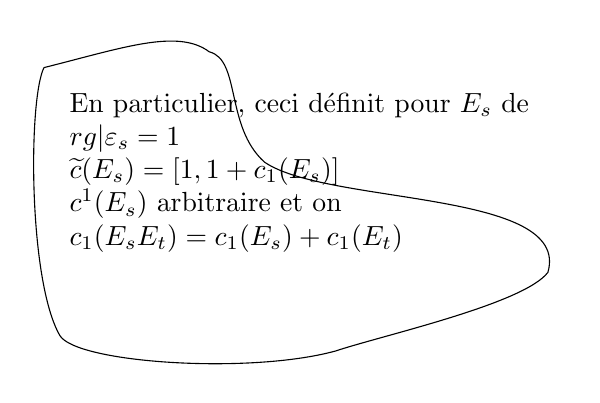
\begin{tikzpicture}[x=1cm,y=1cm]
\node[anchor=north west,align=left,text width=6cm] at (.2,-.1) {En particulier, ceci définit pour $E_s$ de $\unsure{\operatorname{rg}|\varepsilon_s}=1$\par
$\widetilde c(E_s)=[1,1+c_1(E_s)]$\par
$c^1(E_s)$ \unsure{arbitraire} et \deleted{\unsure{on}}\par
$c_1(E_s E_t)=c_1(E_s)+c_1(E_t)$};
\draw (0,.1) .. controls (1,.35) and (1.7,.6) .. (2.1,.3)
 .. controls (2.5,.2) and (2.3,-.65) .. (2.8,-1.1)
 .. controls (3.6,-1.65) and (6.7,-1.45) .. (6.4,-2.5)
 .. controls (6.1,-2.9) and (4.3,-3.3) .. (3.7,-3.5)
 .. controls (2.6,-3.8) and (.4,-3.65) .. (.2,-3.3)
 .. controls (-.2,-2.6) and (-.2,-.3) .. (0,.1);
\end{tikzpicture}}}
\margin{27}
\scanpage{29}
\unsure{noté} $C^*K$, défini par les générateurs
\[
c_{\deleted{\unsure{i}}}^{i}(x)\qquad i\geq1
\]
et les relations
\[
\left\{\begin{array}{ll}
c^i(1)=0 & \text{si }i\geq1,\\
c^n(x+y)=\displaystyle\sum_{i+j=n}c^i(x)c^j(y)&\text{si }x,y\in K,\ n\geq1\\
c^n(x*y)=Q_n(c^1(x),\text{---},c^n(x);c^1(y),\text{---},c^n(y))&\text{pour }x,y\in I(K),\ n\geq1\\
c^n(E_s)=0&\text{pour }n>n_s.
\end{array}\right.
\]
\margin{\unsure{par conséquence des autres relations}}

Noter que l'on a pour tout $E_s$
\[
\gamma^n(E_s-n_s)=0\qquad\text{pour }n>n_s
\]
[en vertu de $\lambda^i(E_s)=0$ pour $i>n_s$] donc les \uline{classes de Chern \unsure{naturelles}} satisfont aux conditions de classes de Chern \deleted{géométriques}\inserted{admissibles} pour les $E_s$, on a donc un hom can
\[
\varphi_K:CK\longrightarrow GK
\]
\[
c^i(x)\rightsquigarrow\gamma^i(x-\varepsilon(x))\mod K^{(i+1)}
\]
évidemment \uline{surjectif} [N.B. plus la famille des $E_s$ est grande, plus on impose des conditions, donc plus $CK$ devient petit, plus on \unsure{peut espérer} demander que $\varphi_K$ soit un \unsure{isom}].

\margin{À voir: la filtration de $K$ définie par les $P(\gamma^i(x-\varepsilon(x)))$ est aussi celle définie par les $P(\gamma^i(E_s-\varepsilon_s))$, [si les $E_s$ engendrent] ???}

\margin{N.B. Il n'y a pas lieu en général, (pour les applications) de \unsure{remplacer} la famille des $E_s$ par l'ens de \unsure{ts les éléments} de $K$ qui sont ``géométriques'', \unsure{car il pourra alors y avoir des} ``bonnes'' applications $\unsure{c_i|c^i}$ telles que $\unsure{c^i\ne0}$ \unsure{pour $i>\varepsilon$}!}

\deleted{D'ailleurs, \unsure{on a tenté de montrer}}
\margin{28}
\scanpage{30}
D'ailleurs, on a déjà noté de nombreuses fois que \unsure{tt} hom de Chern
\[
\unsure{\chi|c}:K\longrightarrow\widetilde A
\]
[qu'il ``respecte'' les $E_s$ ou non] transforme éléments de $K^{(i)}$ en éléments de $A^{(i)}$, d'où un hom naturel \deleted{(additif)}
\[
\psi:\operatorname{Gr}K\longrightarrow\deleted{A}\operatorname{Gr}(\widetilde A)=\unsure{A!|A^!}
\]
\margin{[$\simeq A$ additivement\deleted{]} en degrés $\ne0$]}
\deleted{qui \unsure{est un hom}}

en particulier on a un hom
\[
\psi:\operatorname{Gr}K\longrightarrow\unsure{CK!|CK^!}
\]
\unsure{bien connu} d'ailleurs
\margin{29}
\scanpage{32}
\begin{flushright}
\unsure{Caractères} de Chern\\
covariants, et\\
$\unsure{K^\bullet|K'}$ et $\unsure{A^\bullet|A'}$ \uline{à supports}.
\end{flushright}
\margin{31}
\scanpage{33}
Soit $f:X\longrightarrow Y$ loc. de t.f.

On définit $D_{\mathrm{parf}}(f)$ comme la catégorie \inserted{triangulée} des complexes de $\mathcal O_X$-Modules \uline{parfaits} rel. à $f$, et on définit $K^\bullet_{\mathrm{parf}}(f)$ en conséquence.

Soit $Z\subset X$ un fermé d'un préschéma.

On définit $D_{\mathrm{parf},Z}(X)$ comme la catégorie des complexes de $\mathcal O_X$-modules qui sont parfaits et à cohomologie à support $\subset Z$. D'où aussi $K_Z^\bullet(X)$.
On définit de $=$ $D_{\mathrm{parf},\Phi}(X)$, $K_\Phi^\bullet(X)$, $\Phi$ une ``famille $\Phi$'', \unsure{d'où}
\[
\left\{\begin{array}{l}
\deleted{\unsure{K}}D_{\mathrm{parf},\Phi}(X)=\displaystyle\mathop{\mathrm{Lim}}\limits_{\longrightarrow\atop Z\in\Phi}D_{\mathrm{parf},Z}(X)\\
K_\Phi^\bullet(X)=\displaystyle\mathop{\underline{\lim}}\limits_{Z\in\Phi}K^\bullet_{\unsure{\Phi|Z}}(X),
\end{array}\right.
\]

Soit $i:Z\mathbin{\text{---}}X$ une imm. fermée. On a un foncteur can
\[
\mathrm Ri_*:D_{\mathrm{parf}}(\deleted{\unsure{f}}\inserted{i})\longrightarrow D_Z(X)\qquad\text{d'où}
\]
\[
i_!:K^\bullet(\deleted{\unsure{f}}\inserted{i})\longrightarrow K_Z^\bullet(X)
\]
Soit $\deleted{\unsure{f_n}}i_n:Z_n\longrightarrow X$ le $n$-ième vois. inf. de $Z$ dans $X$, on a alors
\[
\mathop{\mathrm{Lim}}\limits_{\longrightarrow\atop n}D_{\mathrm{parf}}(\deleted{\unsure{f_n}}\inserted{i_n})\longrightarrow D_Z(X)
\]
\uline{le foncteur est pl. fidèle.}
\margin{32}
\scanpage{34}
(\mspage{2}

On a alors un $A$ isomorphisme $A'=A''/J$, où $A''=A\inserted{[t_1,}\ldots t_n\inserted{]}$ et $J$ est un idéal de $A''$. Ecrivant $J$ comme limite inductive de ses sous-idéaux $J_i$ de type fini, et posant $A'_i=A''/J_i$, on aura encore $A'=\mathop{\lim}\limits_{\inserted{\longrightarrow}\atop i}A'_i$ donc $B'$ provient d'une algèbre étale $B'_i$ sur un $A'_i$ (loco citato). D'autre part, comme $\operatorname{Spec}A'\to\operatorname{Spec}A$ est surjectif, il en est de même des $\operatorname{Spec}A'_i\to\operatorname{Spec}A$, de plus on vérifie facilement que puisque $\operatorname{Spec}A'\to\operatorname{Spec}A$ est radiciel, il en est de même de $\operatorname{Spec}A'_i\to\operatorname{Spec}A$ pour $i$ assez grand (appliquer EGA IV 1.9.9. à $\operatorname{Spec}A$). Cela nous ramène au cas où $A'$ est un des $A'_i$, donc de présentation finie sur $A$.

Cela prouve la première assertion de 2.1. Le fait que $f_*$ et $f^*$ soient des équivalences quasi-inverses l'une de l'autre en résulte aussitôt.

\uline{Corollaire} 1.2. Soient $F$ un faisceau abélien sur $X$, $F'$ son image inverse sur $X'$, alors les homomorphismes canoniques
\[
(*)\qquad H^i(X,F)\longrightarrow H^i(X',F')
\]
sont des isomorphismes. De même si $F'$ est un faisceau abélien sur $X'$, $F$ son image sur $X$, les homomorphismes canoniques $(*)$ sont des isomorphismes.

\inserted{\uline{Exemples}}
1.3. Voici des exemples d'application fréquents de 1.1. :

\margin{\figure{\begin{tikzpicture}[x=1cm,y=1cm]
\node[draw,ellipse,rotate=23,align=center] (n) at (0,0) {\unsure{laisser blancs}};
\draw (0.9,0.5)--(1.8,0.85)--(2.15,0.85)--(2.15,1.15)--(2.55,1.15);
\draw (1,0)--(1.8,-0.25)--(2.15,-0.25)--(2.15,0.05)--(2.55,0.05);
\draw (0.8,-0.45)--(1.8,-1.5)--(2.15,-1.5)--(2.15,-1.2)--(2.55,-1.2);
\end{tikzpicture}}}

a) $X'$ est un sous-préschéma de $X$ ayant même ensemble sous-jacent que $X$, i.e. défini par un nil-Idéal $I$.

b) $X$ est un préschéma sur un corps séparablement clos $k$, $k'$ est une clôture algébrique de $k$, et $X'=X\otimes_k k'$.

\deleted{\uline{\unsure{Remarques}}} c) Soit $X$ un préschéma géométriquement unibranche (par exemple une courbe algébrique sur un corps $k$, n'ayant comme singularités que des singularités ``cuspidales'', à l'exclusion en particulier de points doubles ordinaires). Alors, si $X'$ est le \unsure{normalis}
\margin{33}
\scanpage{35}
Définir $K^\bullet_\Phi(X)$\quad ($X$ préschéma.).

Définir un substitut de l'anneau de Chow
\[
\unsure{A}^\bullet_\Phi(X)
\]
(qui doit être un \inserted{pseudo}anneau \unsure{comm.} \inserted{(pas néc d'élément $1$) et une \unsure{flèche} vers $A^\bullet(X)$, l'anneau de Chow ``ordinaire'' \unsure{whitney th.\ + unaires|whitney th.\ + unitaires}]} et des classes de Chern
\[
c^i_\Phi:K^\bullet_\Phi(X)\mathbin{\text{---}}A_\Phi(X)\qquad\boxed{i>0}
\]
qui doit satisfaire la condition de multiplicativité ordinaire interne
\[
\unsure{c^n_\Phi}(x+y)=c^n_\Phi(x)+c^n_\Phi(y)+\sum_{p+q=n\atop p,q>0}c^p_\Phi(x)c^q_\Phi(y)
\]
$(x,y\in K^\bullet_\Phi(X))$, et \deleted{\unsure{pourront}} être compatibles avec \deleted{des} les hom \deleted{\unsure{can}} can.
\diagram{\begin{tikzcd}
K^\bullet_\Phi(X)\arrow[r,"i"]\arrow[d,dash,"c_\Phi"'] & K^\bullet(X)\arrow[d,"c"]\\
A^\bullet_\Phi(X)\arrow[r,"j"] & A^\bullet(X)
\end{tikzcd}}
où la dernière est un hom multiplicatif (canonique).

Cas \inserted{particuliers} à \deleted{\unsure{distinguer}} étudier

1) $X$ est lisse qu.\ pr. sur un corps $k$, \unsure{on prend la} définition habituelle de l'équivalence rationnelle, mais en prenant tjrs des cycles sur $X$ à support $\unsure{\subset|\in}\Phi$.

2) $X$ général: on essaiera de définir $A^\bullet_\Phi(X)$ via une filtration sur le $\lambda$-pseudo-anneau $K^\bullet_\Phi(X)$ ??

3) Classes de Chern \unsure{cohomologiques|homologiques} ??
\margin{34}
\scanpage{36}
\deleted{
Les énoncés 5.7. à 5.\inserted{10}. se généralisent en des énoncés correspondants pour les $\operatorname{Ext}^i$ de faisceaux de Modules, grâce à VI\inserted{,\S}6\inserted{,}5.7., que nous nous dispensons de répéter dans le cas particulier présent. Nous allons par contre expliciter, pour références ultérieures, les variantes de 5.8. et 5.9. en termes de foncteurs $R^nf_{\inserted{*}}$ (VI\inserted{\S}6\inserted{,}4.\inserted{8}.):

\uline{Corollaire} 5.\inserted{11}. Soient $I$ un ensemble \deleted{\unsure{filtrant|filtré}} préordonné filtrant croissant, \inserted{$(X_i)_{i\in I}$ et} $(Y_i)_{i\in I}$ \inserted{deux} \unsure{systêmes|systèmes} projectifs de préschémas, à morphismes de transition affines, \inserted{$X=\varprojlim_i X_i$, $Y=\varprojlim_i Y_i$, $(f_i)_{i\in I}$ un système projectif de \inserted{morphismes $f_i:X_i\longrightarrow Y_i$ \deleted{\unsure{,}} quasi-compacts et quasi-séparés,}} $i_0\in I$, \deleted{$X_{i_0}$ un $Y_{i_0}$-préschéma tel que le morphisme structural \deleted{\unsure{$f_{i_0}$}} $f_{i_0}:X_{i_0}\longrightarrow Y_{i_0}$ soit quasi-compact et quasi-séparé,} $F_{i_0}$ un faisceau sur $X_{i_0}$. Pour tout $i\inserted{\geq}i_0$, \deleted{\unsure{en}} soit \deleted{$f_i:X_i\longrightarrow Y_i$ déduit de $f_{i_0}$ par le changement de base $t_{i_0i}:Y_i\longrightarrow Y_{i_0}$, et} $F_i$ le faisceau sur $X_i$ image inverse de $F_{i_0}$. \deleted{\unsure{on}} Soit de même $f:X\inserted{\longrightarrow}Y$ déduit de $\inserted{(}f_{i\deleted{0}}\inserted{)}$ \deleted{par le changement de base $Y\longrightarrow Y_{i_0}$}, et $F_{\deleted{\unsure{i}}}$ le faisceau sur $X$ image inverse de $F_{i_0}$. Sous ces conditions, l'homomorphisme canonique
\[
\mathop{\lim}\limits_{\inserted{\longrightarrow}\atop\inserted{i}}\inserted{u_i^*}\inserted{(}R^nf_{i\inserted{*}}(F_i)\inserted{)}\inserted{\longrightarrow}R^nf_{\inserted{*}}(F)
\]
est un isomorphisme. \inserted{(où $u_i:X\longrightarrow X_i$ est le morphisme canonique).}

On peut supposer que $i_0$ est un plus petit objet de $I$, et la question étant locale sur $X_{i_0}$, que $Y_{i_0}$ est affine, de sorte que \deleted{\unsure{les}} les $Y_i$ et les $X_i$ sont quasi-compacts et quasi-séparés. On est alors sous les conditions d'application de VI\inserted{,\S}6\inserted{,}4.7.\inserted{,} (o\inserted{ù} on se ramène à 5.8. compte tenu du calcul des $R^nf_{\inserted{*}}$ comme faisceaux associés à des préfaisceaux, V \deleted{\unsure{\S}}\unsure{5.1.}(3)). On prouve de même;

\uline{Corollaire} 5.\inserted{12}. Même énoncé que 5.10., à cela près que maintenant $F_{i_0}$ désigne un préschéma en groupes commutatifs localement de présentation finie sur $X_{i_0}$, et $F_i,F$ ses images réciproques (aux sens du changement de base pour les préschémas).

On fera attention que 5.9. (resp.5.11.) n'est pas un cas particulier de 5.8. (resp.5.10.), cf 2 a) remarque a).
}
\margin{\figure{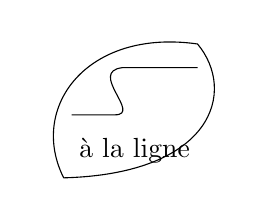
\begin{tikzpicture}[x=1cm,y=1cm]
\draw (-0.8,0.1)--(-0.25,0.1)..controls(0.1,0.1)and(-0.6,0.65)..(-0.15,0.7)--(0.8,0.7);
\node at (0,-0.35) {à la ligne};
\draw (-0.9,-0.7)..controls(-1.35,0.2)and(-0.6,1.2)..(0.8,1)..controls(1.3,0.4)and(1.0,-0.65)..(-0.9,-0.7);
\end{tikzpicture}}}
\margin{35}
\scanpage{37}

On veut les \unsure{variances} habituelles \unsure{raisonnables} sur les \(K^\bullet_\Phi(X), A^\bullet_\Phi(X)\) (images inverses sans conditions (?), images directes \deleted{\unsure{moyen}} \unsure{pour}) (\unsure{morphismes} parfaits) et conditions de propreté des supports.

Utilisant ces constructions, on doit alors, via ``\unsure{bivification|homification}'', définir des \(K^{\Phi}_{?}(X/S)=K^{\Phi}_{?}(f)\) \unsure{covariants} relatifs, ainsi que \(A^{\Phi}_{?}(X/S)=A^{\Phi}_{?}(f)\), et \deleted{\unsure{des}} \inserted{``caractères''} de Chern ``covariants'' \deleted{\(\unsure{C^*_?}\)}
\[
\operatorname{ch}^{X,\Phi}_{?}:K_{?}(X/S)\mathbin{\text{---}}A_{?}(X/S),
\]
\deleted{\unsure{ayant une}} les \(K^{\Phi}_{?}(X/S),\inserted{A^{\Phi}_{?}(X/S)}\) covariants en \(X\) moyennant hyp. de propreté sur supports (\uline{sans plus}), et \(\operatorname{ch}^{X}\) \unsure{vérifie}
\[
\operatorname{ch}^{Y/S}_{?}(g_{?}(x))=g_*(\operatorname{ch}^{X/S}_{?}(x))
\]
\deleted{\[
\unsure{f^X_*}(\qquad g_{?}(\operatorname{ch}^{X}_{?}(x))=\operatorname{ch}^{\unsure{Y}}_{?}(
\]}
i.e. compatible sans plus avec image directe.

Mais R.R. s'interprète comme donnant dans certains cas [\(X/S\) parfait \(\ldots\)] un calcul de \deleted{l'image de} \(\operatorname{ch}^{X/S}_{?}\), comme image
\figure{\begin{tikzpicture}[baseline=(a.base)]
\node[anchor=west,inner sep=1pt] (a) at (0,0) {d'un élément};
\node[draw,ellipse,inner sep=3pt] (b) at (4.0,0) {canonique};
\node[anchor=west,inner sep=1pt] at (5.2,0) {explicitable};
\draw (0,-.05)--(0,.48)--(2.65,.48)--(2.8,.32);
\end{tikzpicture}}
de \(K^\bullet(X)\), par \(K^\bullet(X)\mathbin{\text{---}}K_{?}(X/S)\), en utilisant la structure d'anneaux de \(\unsure{K^\bullet_S(X)|K^\bullet(X)}\) \(\mathbin{\text{---}}\)

\margin{36}
\scanpage{38}

\margin{\deleted{\unsure{module}} \inserted{``algèbre''} sur \(K^\bullet(X')\) (\unsure{pas néc. avec 1})}

\diagram{\begin{tikzcd}[column sep=large,row sep=huge]
K^\bullet(\unsure{i_0|i_\bullet})
  \arrow[r,"{\begin{array}{c}\text{surj. si }X'\text{ régulier}\\u\end{array}}"]
  \arrow[d,"\alpha","{\text{iso si }X'\text{ rég.}}"']
& \underline{\lim}\,K^\bullet(i_n)
  \arrow[r,phantom,"\simeq"]
  \arrow[d,"\beta"',"{\text{iso si }X'\text{ rég.}}"]
& K^\bullet\varinjlim D^\bullet_{\mathrm{parf}}(i_n)
  \arrow[r,"\sim"]
& K^\bullet_X(X')
  \arrow[r,dash,"w"]
  \arrow[d,"\gamma"',"{\text{iso si }X'\text{ rég.}}"]
  \arrow[dll,bend left=27,"\unsure{v}",start anchor=south west]
& K^\bullet(X')
  \arrow[d,"\delta"',"{\text{iso si }X'\text{ rég.}}"]
\\
K_\bullet(X_0)
  \arrow[r,dash,"{\begin{array}{c}u'\\\text{surj. si }X'\text{ rég.}\end{array}}"']
& \varinjlim K_\bullet(X_n)
  \arrow[rr,"w'\ \sim"]
  \arrow[urr,"\deleted{\unsure{v'}}"]
&
& K_\bullet^X(X')
  \arrow[r,"w'"']
  \arrow[ll,bend left=28,"\deleted{\unsure{v'}}"']
& K_\bullet(X')
\end{tikzcd}}

\[
w'v'=\operatorname{id}\qquad
v'w'=\operatorname{id}
\]
\deleted{\(\unsure{\rho\sim\operatorname{id}}\)}

\[
\operatorname{ch}(i_!x)\operatorname{Todd}(X'/S)\qquad X'/S
\]
\figure{
\begin{tikzpicture}[x=.65cm,y=.65cm]
\draw (0,0)..controls (.2,1.6) and (.4,2)..(.1,.4)
..controls (-.1,-.2) and (.8,.5)..(.7,1.8)
..controls (.4,2.3) and (.6,-.5)..(1.3,.7)
..controls (1.8,2.2) and (1.2,2.1)..(1.1,.2)
..controls (1.3,-.6) and (2,1.4)..(1.8,1.9)
..controls (1.6,2.6) and (1.7,.2)..(2.1,.5);
\draw (0,0)--(.8,2) (.35,0)--(1.3,2.1) (.7,-.1)--(1.7,2) (1.1,0)--(2.05,1.8);
\draw (.7,1.5)--(1.2,1.5) (.7,1.2)--(1.15,1.2) (1.1,.6)--(1.6,.6);
\end{tikzpicture}}

\uline{Filtration sur} \(K^\bullet_X(X')\)

\margin{37}
\scanpage{39}

\deleted{
\uline{Corollaire} 5.13. Avec les notations de 5.11. , soit \(F\) un faisceau en groupes abéliens sur \(X\). Alors \deleted{\unsure{le|l'}}\inserted{les} homomorphismes canoniques
\[
\mathop{\operatorname{lim}}\limits_{\inserted{\longrightarrow}\,i}v_i^{\inserted{*}}(R^nf_{i\inserted{*}}(u_{i\inserted{*}}(F)))\inserted{\longrightarrow}R^nf_{\inserted{*}}(F)
\]
sont des isomorphismes\inserted{, (où \(u_i:\unsure{X}\to X_i\) et \(v_i:Y\to Y_i\) sont les homom. canoniques)}.

La démonstration est essentiellement la même que précédemment.
}

\margin{38}
\scanpage{40}

\begin{flushright}
\uline{R.R. des surfaces}

\uline{et autres cas}

\uline{particuliers}

\uline{divers}

\end{flushright}
\margin{39}
\scanpage{41}

\(f:X\longrightarrow Y\) morphisme propre

\diagram{\begin{tikzcd}[row sep=large,column sep=large]
K(X)\arrow[r,"f_!"]\arrow[d,"\widetilde C_X"']&K(Y)\arrow[d,"\widetilde C_Y"]\\
\widetilde A(X)\arrow[d,"h_X"']&\widetilde A(Y)\arrow[d,"h_Y"]\\
A(X)\otimes\mathbb Q\arrow[d,"\tau_h(X)\mathbin{\cdot}"']&A(Y)\otimes\mathbb Q\arrow[d,"\tau_h(Y)\mathbin{\cdot}"]\\
A(X)\otimes\mathbb Q\arrow[r,"f_*"']&A(Y)\otimes\mathbb Q
\end{tikzcd}}
\[
\boxed{\tau_h(Y)\varphi_Y(f_!(\xi))=f_*(\tau_h(X)\varphi_X(\xi))}\tag{1}
\]

\uline{Exemples}

1) \(f\) une injection. \uline{Il y a alors une formule meilleure}, donnant
\[
\boxed{C^j_Y(f_!(\xi))=f_*\left[\frac{C^{q+j}_{\deleted{\unsure{X}}}(\deleted{\unsure{\xi}}\widetilde C(\xi)*\lambda_{-1}(\widetilde C(T_{Y/X})))}{(-1)^q C^q_Y(T_{Y/X})}\right]}\tag{2}
\]
\deleted{\unsure{et}} \unsure{et}

et (1) prend la forme
\[
\boxed{\varphi_Y(f_!(\xi))=f_*(\varphi_X(\xi)\tau_h(T_{Y/X})^{-1})}\tag{1bis}
\]

Noter qu'ici \(f_!(\unsure{\gamma_X(F)|\sigma_X(F)})=\gamma_Y(F)\).

2) \(f\) est une application fibrée. Supposons \(E\) fibré vectoriel sur \(X\), alors on a
\[
f_!(\gamma_X(E))=\sum(-1)^i\cdot\gamma_Y(E^{(i)})
\]
où \(E^{(i)}\) est le fibré vectoriel sur \(Y\) dont la fibre est le \(i\)ième groupe de cohomologie de la fibre de \(X\to Y\).

On a donc \(\varphi_Y(f_!(\gamma_X(E)))=\sum(-1)^i\varphi_Y(E^{(i)})\). Dans le cas où \(E^{(i)}=0\) pour \(i>0\) (p.ex. il en est ainsi si on remplace \(E\) par \(E(n)\) \inserted{\(n\) grand}, provenant d'une immersion de \(X\) comme loc. fermé dans un espace projectif) on détermine ainsi \(\varphi_Y(E^{(0)})\) donc \(\widetilde C_Y(E^{(0)})\) \unsure{mod. la torsion}\deleted{\(\unsure{\xi}\)}. \deleted{\unsure{Si on}} \unsure{On a} dans la formule

\margin{R}
\figure{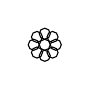
\begin{tikzpicture}[scale=.2]\draw (0,0) circle (.35);\foreach \a in {0,45,...,315}{\draw (\a:.7) circle (.35);}\end{tikzpicture}}
\margin{ARGENTINA LINEN TYPEWRITER}
\figure{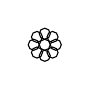
\begin{tikzpicture}[scale=.2]\draw (0,0) circle (.35);\foreach \a in {0,45,...,315}{\draw (\a:.7) circle (.35);}\end{tikzpicture}}
\margin{\unsure{A}}
\margin{40}
\scanpage{42}

\[
\boxed{\tau_h(Y)\sum(-1)^i\varphi_Y(E^{(i)})=f_*(\tau_h(X)\cdot\varphi_X(E))}\tag{1ter}
\]

Prenant les \uline{augmentations} des deux mbs, la formule se réduit essentiellement à R.R. \uline{usuel} (\(Y\) réduit à un point !) sur la fibre. En effet, \unsure{la question étant locale}, le mb de gauche est égal à
\[
\sum(-1)^i\operatorname{rg} E^{(i)}=\chi(Z;E|Z)
\]
(\(Z\) étant une fibre de \(X\to Y\)), le mb de droite est égal aussi à
\[
\unsure{K_p|\kappa_p}\bigl(i^*[(\tau_h(X)\cdot\varphi_X(E))^{(p)}]\bigr),
\]
où \(i:Z\mathbin{\text{---}}X\) est l'application identique, et où \(p\) est la dimension de la fibre, et \({}^{(p)}\) signifie qu'on prend la composante de degré \(p\). On a
\[
\begin{aligned}
i^*[\quad]&=i^*(\tau_h(X))\deleted{\unsure{\varphi}}\cdot i^*(\varphi_X(E))\\
&=\tau_h(C_Z(i^*(T_X)))\varphi_Z(i^*(E))\\
&=\tau_h(C_Z(T_Z))\varphi_Z(E|Z)=\tau_h(Z)\varphi_Z(E|Z).
\end{aligned}
\]
On obtient bien \inserted{\unsure{exactement}} la formule de Hirzebruch pour la fibre. --- Mais prenant des \deleted{\unsure{ci-dessus}}\inserted{composantes} de degré \(\geq1\) des deux mbs, on détermine les classes de Chern (mod torsion) de \(\sum(-1)^iE^{(i)}\) (donc, en certains cas) de \(E^{(0)}\), ce qui n'est pas contenu dans la formule de Hirzebruch proprement dite. On trouve \unsure{en passant} le résultat suivant (qui n'est pas non plus trivial): \uline{pour \(n\) grand}, \uline{la classe de Chern modifiée de} \(E(n)^0=f_*(E(n))\) \uline{dépend polynomialement}

\margin{\unsure{peut aussi se déduire dans le cas général}}
\margin{41}
\scanpage{43}

\uline{de \(n\)}. En effet, on a
\[
\varphi_X(E(n))=\varphi_X(E)\deleted{\unsure{\varphi}}e^{n\xi}.
\]
d'où
\[
\tau_h(X)\varphi_X(E(n))=\underbrace{\tau_h(X)\varphi_X(E)}e^{n\xi}=\sum_k n^k\left[\frac{\xi^k}{k!}\tau_h(X)\varphi_X(E)\right]
\]
et
\[
f_*(\tau_h(X)\varphi_X(E(n))=\sum_k n^k f_*\left(\frac{\xi^k}{k!}\tau_h(X)\varphi_X(E)\right)
\]

\figure{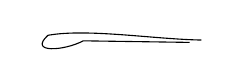
\begin{tikzpicture}[x=1cm,y=1cm]\draw (0,0)..controls (-.25,-.23) and (.2,-.2)..(.45,-.07)--(1.8,-.09);\draw (0,0)..controls (.5,.09) and (1.35,-.05)..(1.95,-.06);\end{tikzpicture}}

Cas de morphisme propre quelconque.

1) Morphisme d'une courbe \deleted{\(\unsure{Y}\)} \inserted{\unsure{nons. complète|irr. complète}} \(X\) dans une variété \(X\).

On peut évidemment supposer \(f\) non constant, \(X\) et \(Y\) irréductibles.

\deleted{\unsure{X et Y irréductibles}}

On a \(K(\unsure{X})\simeq\mathbb Z+\mathfrak P(\unsure{X})\), \unsure{un} l'isomorphisme étant précisément donné par la application \deleted{\(\unsure{C}\)}\(\widetilde C\) de Chern. On doit donc \deleted{\unsure{définir}}\inserted{calculer}, pour \(\xi=(n,d)\) son image \(f_!(\xi)\in K(Y)\) en fonction de \(n,d\). Noter que \(\varphi_X(\xi)=n+\underline d\), \(\widetilde C(T_X)=(1,-\underline k)\) donc \(\tau_h(X)=\frac{-\underline k}{1-e^{\underline k}}=\unsure{1-\tfrac12\underline k|1\,\tfrac12\underline k}\), \(\underline k\) étant la classe canonique. Donc

\deleted{a) \(X\) est courbe (non singulière irréductible).}
\[
\varphi_X(\xi)\tau_h(\unsure{X})=(1-\tfrac12\underline k)(n+\underline d)=\deleted{\unsure{n+\underline d+\underline k}}n+(\underline d-n\tfrac12\underline k)
\]

 a) \(Y\) est une courbe. Soit \(\underline{k'}\) son diviseur canonique d'où \(\tau_h(Y)=1-\tfrac12\underline{k'}\). Soit \(\delta\) le \uline{degré} de \(f\).

alors on a \(f_*(1)=\delta\), donc
\[
f_*(\varphi_X(\xi)\tau_h(X))=n\delta+\left(f_*(\underline d)-nf_*(\tfrac12\underline k)\right)
\]
d'où
\[
\begin{aligned}
\varphi_X(f_!(\xi))&=\tau_h(Y)^{-1}f_*(\mathord{\cdot}\mathbin{\text{---}})=(1+\tfrac12\underline{k'})(n\delta+(f_*(\underline d)-nf_*(\tfrac12\underline k)))\\
&=n\delta+\left[n\delta\tfrac12\underline{k'}+f_*(\underline d)-nf_*(\tfrac12\underline k)\right]
\end{aligned}
\]
par suite
\[
\boxed{f_!(\xi)=\left(n\delta,\ n\delta\tfrac12\underline{k}_Y+f_*(\underline d)-nf_*(\tfrac12\underline{k}_X)\right)}\qquad(f:x\longrightarrow Y)
\]

\margin{R}
\figure{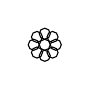
\begin{tikzpicture}[scale=.2]\draw (0,0) circle (.35);\foreach \a in {0,45,...,315}{\draw (\a:.7) circle (.35);}\end{tikzpicture}}
\margin{ARGENTINA LINEN TYPEWRITER}
\figure{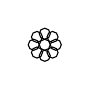
\begin{tikzpicture}[scale=.2]\draw (0,0) circle (.35);\foreach \a in {0,45,...,315}{\draw (\a:.7) circle (.35);}\end{tikzpicture}}
\margin{A}
\margin{42}
\scanpage{44}

p.ex. Si \(\deleted{\unsure{f}}\inserted{X}\) est un revêtement ramifié (séparable ou non) de degré \(\delta\) de \(Y\) par \(f\), alors \(f_*(\underline O_X)\) est un \deleted{\unsure{fibré}} faisceau sur \(X\) correspondant à un fibré \deleted{\unsure{loc.}} de \deleted{degré} rang \(\delta\), et dont la classe de Chern est
\[
\tfrac12\deleted{\unsure{n}}(\delta\underline k_Y-f_*(k_X))
\]

b) \(Y\) est une surface non singulière. Soient \(k_Y^{\unsure{1|' }}\) et \(\unsure{k_Y^2}\) les deux \deleted{classes de Chern du fibré tangent}\inserted{\unsure{canoniques}} \deleted{dont \(k_Y^{(1)}\) est la classe canonique, \(k_Y^2\) est \unsure{la classe de Euler|la classe de Chern}}. On a
\[
C(T_Y)=1-k_Y^1+\unsure{k_Y^2}
\]
donc
\[
\tau_h(Y)=1-\tfrac12k'_Y+\underbrace{\deleted{\unsure{\tfrac1{12}((k'_Y)^2+k_Y^2)}}}
\]
et par suite
\[
\tau_h(Y)^{-1}=1+\tfrac12k'_Y+\deleted{\unsure{\tfrac1{12}((k'_Y)^2+k_Y^2)}+\tfrac14(k'_Y)^2=1+\tfrac12k'_Y+\tfrac1{12}[\unsure{k_Y^2-2(k'_Y)^2}]}
\]
\[
f_*(1)=\delta f(X)=\delta C
\]
\deleted{\unsure{où}}\inserted{où \(C\) est l'image} de \(X\) considérée comme classe de diviseurs, et \(\delta\) le degré de \(X\to C\)

\(f_*(\underline k_X),f_*(\underline d)\): classes de \(0\)-cycles.

\[
\varphi_Y(f_!(\xi))=[1+\tfrac12k'_Y\deleted{\unsure{-\tfrac1{12}((k'_Y)^2-2k_Y^2)}}\inserted{+}\ ][\deleted{\unsure{n\delta}}\inserted{n\delta C}+(f_*(\underline d)-\tfrac12n f_*(\underline k_X))]
\]
\[
\boxed{\varphi_Y(f_!(\xi))=n\delta C+\left[f_*(\underline d)-\tfrac12n f_*(\underline k_X)+\tfrac12n\delta C.K_Y\right]}
\]
\[
\begin{aligned}
C_Y(f_!(\xi))&=\exp[n\delta C\unsure{\underset{1}{-}|-\tfrac11}[\qquad]\,)\\
&=1+n\delta C-[\quad]+\tfrac12n^2\delta^2C^2
\end{aligned}
\]
d'où
\[
\boxed{C_Y(f_!(\xi))=1+n\delta C+\left[\tfrac12n^2\delta^2C^2-\tfrac12n\delta C K_Y-f_*(\underline d)+\tfrac12n f_*(K_X)\right]}
\]
Supposons \(n=\delta=1\) \deleted{\unsure{et}} on trouve
\[
C_Y(f_!(\xi))=1+C+\left[\tfrac12(C^2-CK_Y)-f_*(\underline d)+\tfrac12f_*(k_X)\right]
\]

\margin{43}
\scanpage{45}

En particulier, on trouve la deuxième classe de Chern d'une courbe \(C\) dans la surface \(Y\):
\[
C^2(\underline O_C)=\tfrac12[C^2-CK_Y+f_*(k_{\unsure{\widetilde C|C}})]
\]
où \(f:\widehat C\mathbin{\text{---}}Y\) est l'homomorphisme canonique dans \(Y\) de la normalisée \(\widetilde C\) de \(C\), et \(k_{\widetilde C}\) la classe canonique sur \(\widetilde C\). Si \(Y\) est compacte, et \(\widetilde C\) de genre \(g\), on trouve, en prenant les \(\unsure{K_2|\kappa_2}\) des deux mbs
\[
\unsure{K_2|\kappa_2}(C^2(\underline O_C))=\tfrac12[C^2-CK_Y+2g-2]=\tfrac12(C^2-CK_Y)+g-1
\]

\margin{PEWRITER}
\figure{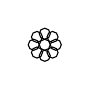
\begin{tikzpicture}[scale=.2]\draw (0,0) circle (.35);\foreach \a in {0,45,...,315}{\draw (\a:.7) circle (.35);}\end{tikzpicture}}
\margin{ARGENTINA LINEN \unsure{TYPEWRI}}
\margin{44}
